\documentclass[en, msc, classic, a4paper]{ifbathesis}

%% Preambulo:
\usepackage[utf8]{inputenc}
\usepackage[english]{babel}
\usepackage{graphicx}
\usepackage{lipsum}
\usepackage{hyphenat}
% \usepackage[usenames, dvipsnames, table]{xcolor}
\usepackage{float}
\usepackage{booktabs}
\usepackage{pifont}
\usepackage{multirow}
\usepackage{listings} 
\usepackage{colortbl}
\usepackage{xfrac}
\usepackage{nameref}
\usepackage{cleveref}
\usepackage[FIGTOPCAP]{subfigure}
\usepackage[printonlyused, withpage]{acronym}
\usepackage{graphicx,url}
%\usepackage[hidelinks,breaklinks]{hyperref}
%\PassOptionsToPackage{hyphens}{url}
\usepackage{makecell}
\renewcommand\theadfont{\bfseries\sffamily}
\usepackage{minted}
\usepackage[table]{xcolor}% http://ctan.org/pkg/xcolor

% ADD SUBSUBSUBSECTION
\newcommand{\subsubsubsection}[1]{\paragraph{#1}\mbox{}\\}
\setcounter{secnumdepth}{4}
\setcounter{tocdepth}{4}

\newenvironment{dedication}
  {\clearpage           % we want a new page
   \thispagestyle{empty}% no header and footer
   \vspace*{\stretch{6}}% some space at the top 
   \itshape             % the text is in italics
   \raggedleft          % flush to the right margin
  }
  {\par % end the paragraph
   \vspace{\stretch{0}} % space at bottom is three times that at the top
   \clearpage           % finish off the page
  }
  
\university{Instituto Federal da Bahia}
\address{Salvador}
\institute{Departamento de Pós-Graduação e Qualificação}
\library{Biblioteca Professor Raul Varella Seixas}
\program{Programa de P\'{o}s-Gradua\c{c}\~{a}o em Engenharia de Sistemas e Produtos}
\majorfield{Engenharia de Sistemas e Produtos}
\title{A blockchain framework for traceability in supply chain management}

% Data da defesa
% e.g. \date{19 de fevereiro de 2013}
\date{15 de maio de 2021}
% e.g. \defenseyear{2013}
\defenseyear{2021}

% Autor
\author{Edivaldo Mascarenhas Ferreira de Jesus Júnior}

% Orientador(a)
\adviser{Manoel Carvalho Marques Neto}
\coadviser{Allan Edgard Silva Freitas}

%% Inicio do documento
\begin{document}
\ppgespfrontpage
\frontmatter
\ppgesppresentationpage

\begin{dedication}
\vspace*{\fill}
    This work is dedicated to the memory of \\ Edivaldo M. F. de Jesus (1951--2021)
    \vspace*{\fill}

\end{dedication}

%%%%%%%%%%%%%%%%%%%%%
% Resumo em Portugues
%%%%%%%%%%%%%%%%%%%%%

\resumo
Os avanços nas tecnologias da informação e comunicação reduziram as barreiras físicas, políticas e culturais entre as nações. Essas tecnologias permitiram a globalização ao acesso de matérias-primas, bens e serviços. A complexa rede de relacionamentos que envolve quem fornece materiais, fabricam componentes ou subprodutos, montam ou misturam as partes e entregam o produto final no mercado é conhecida como cadeia de suprimentos. O rápido crescimento das tecnologias da internet permitiu o surgimento de muitas soluções emergentes aplicadas em sistemas de rastreabilidade, na área da cadeia de suprimentos. No entanto, esses sistemas tendem a ser centralizados, monopolistas, assimétricos e opacos. Como consequência, essas aplicações estão susceptíveis à problemas de confiança como fraude, corrupção, adulteração e falsificação de informações. Da mesma forma, por ser um ponto único de falha, o sistema centralizado é vulnerável ao colapso. Atualmente, uma emergente tecnologia chamada blockchain apresenta uma nova abordagem baseada na descentralização. No entanto, por estar em seus estágios iniciais, ela tem alguns desafios a enfrentar, nos quais a ratreabilidate a escalabilidade e o desempenho se tornam principalmente um desafio para encarar a enorme quantidade de dados no mundo real. Este trabalho pretende fornecer uma estrutura baseada em blockchain para facilitar o desenvolvimento de aplicações para rastreabilidade no gerenciamento da cadeia de suprimentos.


% Palavras-chave do resumo em Portugues
\begin{keywords}
Blockchain; gerência de cadeia de suprimento; rastreabilidade; contratos inteligentes.
\end{keywords}

%%%%%%%%%%%%%%%%%%%
% Resumo em Ingles
%%%%%%%%%%%%%%%%%%%

\abstract
Advances in information and communication technologies have reduced the physical, political and cultural barriers between nations. These technologies have enabled globalization to access raw materials, goods, and services. The complex web of relationships that provide materials manufacture the components, assemble or mix the parts and deliver the final product to market is known as the supply chain. The rapid growth of internet technologies allowed the onset of many emerging technologies applied in traceability systems, in the supply chain area. However, these systems tend to be centralized, monopolistic, asymmetric, and opaque. Consequently, these systems results in trust problem, such as fraud, corruption, tampering and falsifying information. Likewise, by being a single point of failure, a centralized system is vulnerable to collapse. Nowadays, a new technology called the blockchain presents a whole new approach based on decentralization. Nonetheless, being in its early stages has some challenges to deal with, in which traceability, scalability, and performance become mainly defiance to face the massive amount of data in the real world.  This work is intended to provide a blockchain-based framework to facilitate the development of applications for traceability in supply chain management.

% Palavras-chave do resumo em Ingles
\begin{keywords}
Blockchain; supply chain management; traceability; smart contracts.
\end{keywords}

\tableofcontents
\listoffigures
\listoftables
\chapter*{List of Acronyms}
\begin{acronym}[PPGESP]
    \acro{PPGESP}{Programa de Pós-Graduação em Engenharia de Sistemas e Produtos}
    \acro{CNPq}{Conselho Nacional de Desenvolvimento Científico e Tecnológico}
    \acro{BG}{Byzantine generals}
    \acro{PoW}{proof-of-work}
    \acro{BFT}{Byzantine fault tolerance}
    \acro{SC}{smart contract}
    \acro{SCM}{Supply Chain Management}
    \acro{TAM}{Technology Acceptance Model}
    \acro{SCM-BP}{Supply Chain Management - Blockchain Platform}
\end{acronym}

%% Parte textual
\mainmatter

%Seções
\xchapter{Introduction}{}

% É recomendável utilizar `\acresetall' no início de cada capítulo para reiníciar o contator de referências às siglas.
\acresetall 

Hundreds of years ago, supply chains were fairly simple. Mines and farms provided natural resources to skilled craftsman like blacksmiths and Tailors who then created and sold finished products. Today's supply chains are much more complicated, fragmented and difficult to understand. Hundreds or even thousands of supplies all around the world contribute to make and ship products purchased by a customer. Most of the time the various companies don't know about each other and a final consumer likely don't know anything about how, where, when or under what condition the products passed through. This isn't just a problem for consumers. Today's supply chains are so complex that even big industry players have difficulty tracking how their goods get made.

%{\color{red}adicionar aqui texto sobre o problema atual da cadeia de suprimento.}

In order to solve some problems that come with this complexity, such as supply chain visibility and traceability, many systems have been developed. However, these systems typically store information in standard databases controlled by service providers. This centralized data storage becomes a single point of failure and risks tampering. As a centralized organization, it can become a vulnerable target for bribery, and then the whole system can not be trusted anymore.

Blockchain and smart contracts could make supply chain management simpler and more transparent. The idea is to create a single source of information about products and supply chain via global ledger. Each component would have its own entry on the blockchain that gets tracked over time. Both untrust companies could then update the status of a good in real-time. The end result is once the clients receive their products they could track every piece back to its manufacturer. Theoretically users could trace the supply chain all the way back to the mines where the raw materials came from \cite{greve2018blockchain}.

Companies can also use the blockchain supply chain as a single source of truth for their products. They can manage and monitor risks within the supply chain, ensure quality of delivery parts and track delivery status of all this. Additionally companies can use smart contracts to manage and pay for supply chain autonomously. For example a chip manufacturer it could be paid immediately upon testing of each individual chip at the assembly facility. This would reduce the need for large contract invoices on the back-and-forth of refund requests for faulty components. Those same smart contracts could assist with shipping and logistics tracking valuable products as they travel around the world. Using blockchain, companies can finally have a complete picture of their products at every stage in the supply chain, bringing transparency to the production process while reducing the cost of manufactured goods.

This work presents \acf{SCM-BP}, a generic framework intended to be used in any kind of supply chain correlated to assets and products. Also presents a use case of this framework applied.

This paper is structured as follow: Chapter~\nameref{chap:Theoretical} presents several technologies involved in the preparation of this article, aimed to introduce important concepts of Computer area in which the context of this project is inserted and also presents business concepts related to supply chain management. Chapter~\nameref{chap:RelatedWork} shows correlated works. Chapter~\nameref{chap:Technical} presents the solution and its architecture. Chapter~\nameref{chap:Implementation} exposes details of the executed implementation. Chapter~\nameref{chap:validation} exposes the validation and its results. The last section presents the conclusions.
\xchapter{Theoretical Background}{In this section the main concepts studied are presented, which provided subsidies for the development of the proposed project.}\label{chap:Theoretical}


%\section{General Context}\label{sec:generalContext}



\section{Supply Chain Management}\label{sec:scm}

The complex web of relationships that provide materials manufacture the components, assemble or mix the parts and deliver the final product to market is known as the supply chain \cite{buurman2002supply}.

Management is on the verge of a major breakthrough in understanding how industrial company success depends on the interactions between the flows of information, materials, money, manpower, and capital equipment. The way these five flow systems interlock to amplify one another and to cause change and fluctuation will form the basis for anticipating the effects of decisions, policies, organizational forms, and investment choices \cite{forrester1958industrial}.

The term \ac{SCM} has risen to prominence over the past fifteen years \cite{cooper1997supply}. For example, at the 1995 Annual Conference of the Council of Logistics Management, 13.5\% of the concurrent session titles contained the words "supply chain." At the 1997 conference, just two years later, the number of sessions containing the term rose to 22.4\%. Moreover, the term is frequently used to describe executive responsibilities in corporations \cite{la1997supply}. SCM has become such a "hot topic" that it is difficult to pick up a periodical on manufacturing, distribution, marketing, customer management, or transportation without seeing an article about SCM or SCM-related topics \cite{ross1997competing}.

The definition of supply chain seems to be more common across authors than the definition of "supply chain management" \cite{cooper1993characteristics, la1994emerging, lambert1998fundamentals}. La Londe and Masters proposed that a supply chain is a set of firms that pass materials forward. Normally, several independent firms are involved in manufacturing a product and placing it in the hands of the end user in a supply chain—raw material and component producers, product assemblers, wholesalers, retailer merchants and transportation companies are all members of a supply chain \cite{la1994emerging}. By the same token, Lambert, Stock, and Ellram define a supply chain as the alignment of firms that brings products or services to market. 

Another definition notes a supply chain is the network of organizations that are involved, through upstream and downstream linkages, in the different processes and activities that produce value in the form of products and services delivered to the ultimate consumer \cite{christopher2017logistics}. In other words, a supply chain consists of multiple firms, both upstream (i.e., supply) and downstream
(i.e., distribution), and the ultimate consumer. 

As a summarization, \cite{mentzer2001defining} defines a supply chain as a set of three or more entities (organizations or individuals) directly involved in the upstream and downstream flows of products, services, finances, and/or information from a source to a customer. 


To begin with, the starting point of a supply chain is the extraction of raw materials and how they are first processed (preprocessed) by suppliers for delivery in the next step. The next step is called manufacturing, where the conversion process for raw materials takes place. Following this, the constructed products are passed to the distributors who are responsible for allocating them to multiple different intermediaries, such as wholesalers and retailers. Distributors also maintain an active inventory of products, as previous products are connected to suppliers. Subsequently, wholesalers do not sell products directly to the public, but to other retailers, whereas retailers dispose products purchased to end users. Finally, Consumers are who buy or receive goods or services for personal needs or use and not for commercial resale or trade purposes \cite{litke2019blockchains}.

The manufacturer needs to validate crucial information about the natural resources they collected by reading and verifying all tags that the latter includes in its transactions and then proceeding to the proper execution of manufacturing step. New transactions with new information, such as manufacturer name, field experience and more, are sent after the internship has completed. Then the products are delivered to distributors. Distributors are able to sell products to wholesalers and retailers. This process is represented by transactions that contains important data, such as merchant and customer address, exchange value, product raw material quality, and more \cite{sauer2018extending}. 

As the distributors sell products to intermediates (generally not end users), they must check the information about the progress route until that stage, for example the raw material origin, manufactures company popularity, distributor address and others. Retailers can audit product's natural resource quality, and get the appropriate feedback before selling it to the consumer. After that, when a distributor send the product to the wholesaler, some details, such as manufacturer name, field experience and others, are submitted after the completion of acts in a similar way. Wholesaler needs to check these information and execute their selling to another wholesaler or retailer company. The same applies to the retailer companies. Finally, end users obtain the final product and should able to track and verify all aspects from the beginning of its supply chain journey \cite{litke2019blockchains}. 
\section{Traceability}\label{sec:traceability}

\citeonline{gryna1998juran} define Traceability as the ability to preserve the identity of the products and their origins, so that the collection, documentation and maintenance of information related to all processes in the production chain must be ensured. For a food product, traceability represents the ability to identify where and how it was grown, as well as the ability to track its post-harvest history and to identify the processes performed at each step in the production chain through records. Traceability is required primarily for \cite{horiuchirastreabilidade}:
\begin{itemize}
\item Improve credibility with customers and consumers.
\item Ensure that only quality materials and components are present in the final product.
\item Better allocate responsibilities.
\item Identify products that are distinct but may be confused.
\item Enable the return of defective or suspect products.
\item Find the causes of failures and take steps to repair them at the lowest possible cost.
\end{itemize}

consumers consider traceability as part of an expected protection package when purchasing products. In this scope, the traceability can improve credibility since all the related providers and dealers or other agent between the raw manufactures and the final consumer can be tracked. In a traceability system the responsibility papers are well defined. A traceability system allows any user to track products by providing information about them (eg. originality, components, or locations) during production and distribution. Suppliers and retailers typically require independent, government-certified traceability service providers to inspect products throughout the supply chain. Vendors and retailers request traceability services for different purposes.Suppliers want to receive certificates to showcase their products. Retailers want to verify the origin and quality of products \cite{lu2017adaptable}.


In \cite{opara2003traceability} six important elements are to be considered for traceability:

\begin{itemize}
\item Product Traceability: Determines the location of a product at any stage of the production chain. to facilitate logistics, inventory management, product recall, and information disclosure to consumers and customers.
\item Process Traceability: Identifies the type and sequence of activities that affected a particular product. This includes any interactions between the product and physical / mechanical, chemical and environmental factors that result in the transformation of raw material into value added products.
\item Genetic Traceability: determines the genetic constitution of the product.
\item Input Traceability: Determines the type and source of input such as fertilizers and livestock.
\item Traceability of Diseases and Pests: Tracks the epidemiology of pests such as bacteria and viruses.
\item Measurement Traceability: determines the measurement instruments, in addition to specifying the environmental, geospatial and temporal factors that influence data quality.
\end{itemize}

Supply chain visibility, or traceability, is one of the key challenges encountered in the business world, with most companies having little or no information about their own second- and third-tier suppliers. Transparency and end-to-end visibility of the supply chain can help shape product, raw material, test control, and end product flow, enabling better operations and risk analysis to ensure better chain productivity \cite{abeyratne2016blockchain}.

Folinas et al. \cite{folinas2006traceability} identified that the efficiency of a traceability system depends on the ability to track and trace each individual asset and logistics units, in a way that enables continuous monitoring from firstly processed until final clearance by the consumer.

\citeonline{aung2014traceability} and \citeonline{golan2004traceability} set three main traceability objectives, namely: (1) better supply chain management, (2) product differentiation and quality assurance, and (3) better identification of non-compliant products. An additional objective is to maintain assurance of traceability in accordance with applicable regulations and standards. A complete traceability system will include components that manage \cite{vargas2017trazabilidad}:

\begin{enumerate}
\item Identification, marking and assignment of traceable objects, parties and locations.
\item Automatic capture (by scanning or reading) of movements or events involving an object.
\item Record and share traceability data, internally or with parts of a supply chain, so that visibility of what has occurred can be achieved.
\end{enumerate}

Traceability systems typically store information in standard databases controlled by service providers. This centralized data storage becomes a single point of failure and risks tampering. As consequence, these systems results in trust problem, such as fraud, corruption, tampering and falsifying information. Likewise, by being a single point of failure, centralized system is vulnerable to collapse \cite{tian2017supply}.

Nowadays, a new technology called the blockchain presents a whole new approach based on decentralization. Blockchain enables end-to-end traceability, bringing a common technology language to the supply chain, while allowing consumers to access the assets history of these products through a software application. This characteristic is provided by a immutable register ledger which facilitates the process of recording transactions and tracking assets across a network \cite{galvez2018future}.
\section{Blockchain}\label{sec:blockchain}

Recently, cryptocurrency has attracted extensive attention from both the industry and the academy. Bitcoin, often called the first cryptocurrency, had massive success, with the capital market coming to \$ 10 billion in 2016 \cite{coindesk}. Blockchain is the central mechanism of Bitcoin and was first proposed in 2008 and implemented in 2009 \cite{nakamoto2008bitcoin}. The blockchain can be considered a  public ledger, in which All committed transactions are stored in a block chain. This chain grows continuously when new blocks are attached to it \cite{zheng2016blockchain}.

At the origin of the blockchain is the Bitcoin protocol, proposed by Satoshi Nakamoto \cite{nakamoto2008bitcoin}. This article proposes a  \ac{P2P} network where transactions with the cryptocurrency bitcoin, proposed by customers, are received by servers, who will decide, through a consensus protocol based on cryptographic challenges, on the order in which they will be carried out and permanently stored in a chain of blocks, replicated on each server. According to \citeonline{FORMIGONI2017}, it was the creation of a digital currency that worked in a P2P network that allowed the sending of online payments in a completely secure way, without the involvement of financial institutions, for all participants from the web. In this sense, blockchain was created motivated by an efficient, economical, reliable, and secure system to conduct and record financial transactions. Hence the question: what is the relationship between blockchain and Bitcoin? Blockchain is the platform used for the operation of the Bitcoin network and several other cryptocurrencies.

While the system of financial institutions that serve as third parties reliable processors for processing payments work well for most still suffers from the shortcomings inherent in the model based on confidence. In addition, the cost of mediation increases transaction costs, limiting the minimum practical size of the transaction and eliminating the possibility of occasional small transactions. To solve these problems, \cite{nakamoto2008bitcoin} defined an electronic payment system called Bitcoin based on cryptographic proof rather than reliability, allowing either party to be willing to transact directly without the need for a reliable third party.

This revolution began with a new marginal economy on the Internet. Bitcoin emerges as an alternative currency issued and not backed by a central authority but by automated consensus among networked users. However, its true uniqueness lay in the fact that it did not require that users trust each other. Through self-policing algorithmically, any malicious attempt to circumvent the system would be rejected. In a precise and technical definition, Bitcoin is digital money transacted via the Internet in a decentralized system without bail, using a ledger called blockchain. It is a new way of combining peer-to-peer file sharing rent with public key encryption \cite{swan2015blockchain}.

For \cite{swan2015blockchain}, besides the currency ( "Blockchain 1.0"), smart contracts ("2.0") demonstrate how the blockchain is in a position to become the fifth disruptive computing paradigm after mainframes, PCs, Internet, and mobile/ social networks. Bitcoin is starting to become a digital currency, but the technology blockchain behind it can be much more significant.

The rapid growth in blockchain technology adoption and the development of applications based on this technology have revolutionized financial services industries. In addition to bitcoin, typical applications of blockchain usage vary from proprietary networks used to process financial claims, insurance claims to platforms that can issue and trade equity and corporate bonds \cite{michael2018blockchain}.

Blockchain exists with real-world implementations beyond cryptocurrencies, and these solutions deliver potent benefits to healthcare organizations, bankers, retailers, and consumers. The potential benefits of blockchain are more than just economic. They extend to the political, humanitarian, social, and scientific domains. Specific groups are already harnessing their technological capacity to solve real-world problems \cite{michael2018blockchain}.



\subsection{Blockchain Properties}\label{sec:propriedades}

Blockchain technology has key features such as centralization, persistence, anonymity, and auditability. Blockchain can function in a decentralized environment that is activated by integrating several key technologies such as cryptographic hash, digital signature (based on asymmetric encryption), and distributed consensus engine. With blockchain technology, a transaction may occur in a decentralized manner. As a result, blockchain can significantly save costs and improve efficiency \cite{zheng2016blockchain}. The primary properties of the blockchain are considered innovative and enable rapid adoption for technology \cite{greve2018blockchain}:

\begin{itemize}
\item Decentralization: Applications and systems run in a distributed manner, through the establishment of trust between the parties, without the need for a trusted intermediary entity. This is the primary motivator for the growing interest in the blockchain.
\item Availability and integrity: All datasets and transactions are securely replicated in different nodes to keep the system available and consistent.
\item Transparency and auditability: All transactions recorded in the ledger are public and can be verified and audited. Furthermore, technology codes are often open, verifiable.
\item Immutability and Irrefutability: Transactions recorded in the ledger are immutable. Once registered, they cannot be refuted. Updates are possible based on the generation of new transactions and the realization of a new consensus.
\item Privacy and Anonymity: It is possible to offer privacy to users without the third parties involved having access and control of their data. In technology, each user manages their keys, and each server node stores only encrypted fragments of user data. Transactions are somewhat anonymous, based on the address of those involved in the blockchain.
\item Disintermediation: Blockchain enables the integration between different systems directly and efficiently. Thus, it is considered a connector of complex systems (systems of systems), allowing the elimination of intermediaries to simplify the design of systems and processes.
\item Cooperation and Incentives: Offer of an incentive-based business model in the light of game theory. On-demand consensus is now offered as a service at different levels and scopes.
\end{itemize}


\section{Fundamentals of blockchain}\label{sec:fundamentals}
In this section, the key elements of the blockchain that contribute to its properties will be displayed: integrity, immutability, transparency, availability, disintermediation, decentralization.

\subsection{Cryptography}\label{sec:criptografia}
Blockchain relies heavily on encryption to satisfy system and application security requirements. As the word suggests, cryptocurrencies also make heavy use of encryption. Encryption provides a mechanism for safely encoding the rules of system encryption on the system itself. This can prevent tampering and misconceptions and coding in a mathematical protocol the rules for creating new currency units. So, before understanding blockchains correctly, it is necessary to understand the cryptographic foundations they trust \cite{narayanan2016bitcoin}.

Cryptography is a profound academic field of research that uses many advanced mathematical techniques that are notoriously subtle and complicated. In this chapter, cryptographic hashes and digital signatures will be defined, which stand out among the most used resources. For more details, the reader should refer to the book \cite{narayanan2016bitcoin}.

\subsubsection{Cryptographic Hashes}\label{sec:hashesCriptograficos}
A hash function is a mathematical function with the three properties to be followed \cite{narayanan2016bitcoin}:

\begin{itemize}
\item  Its input can be any string of any length;
\item Produces a fixed size output. To make concrete the discussion in this chapter (e.g., 256 digits);
\item It is efficiently computable. Intuitively, this means that it is possible to find out the hash function output within a reasonable time for a given input string. Technically, hashing a n-bit string must have an $O(n)$ runtime.
\end{itemize}

These properties define a general hash function. Cryptographic hash functions (or cryptographic summaries) are unidirectional and hardly allow retrieving the original value $x$ from the hash $h$. For a hash function to be cryptographically secure, it must satisfy the following three properties: (1) collision resistance, (2) hiding, and (3) puzzle friendliness \cite{greve2018blockchain}.

A collision occurs when two distinct inputs produce the same output. A hash function $H$ is collision-resistant when it is impossible to find two values $x$ and $y$, such that $x \neq y$ and $H(x) = H(y)$ \cite{narayanan2016bitcoin}.

The hidden property states that having the hash function output $y = H (x)$, there is no possible way to find the $x$ input \cite{greve2018blockchain}.

A hash function $H$ is considered puzzle friendliness if for each possible output value of $n$ bits $y$ if $k$ is chosen from a distribution with high min-entropy, then it is impracticable to find $x$ such that $H (k \| x) = y$ in time significantly less than $2^n$ \cite{narayanan2016bitcoin}.

\subsubsection{Digital Signatures}\label{sec:assinaturasDigitais}
A digital signature is supposed to be a digital analog of a handwritten paper signature. Two signature properties are desired, which correspond well to the analogy of the handwritten signature. First, only one person can make their signature, but anyone can verify if it is valid. Secondly, it is desired that the signature be linked to a specific document, so it cannot indicate the agreement or endorsement to a different document \cite{merkle1989certified}. Moreover, it is not possible to forge a signature in such a way as to reuse it in some other context. That is, signatures must be irrefutable.

To implement digital signatures, asymmetric key encryption is used. A secret key (sk) is used for signing the document, and a public key (pk) is used to attest the signature's authenticity \cite{greve2018blockchain}.

A digital signature consists of the following three algorithms \cite{narayanan2016bitcoin}:

\begin{itemize}
\item $(sk , pk) := generateKeys(keysize)$ – The $generateKeys()$ method receives a key size $(keysize)$ in the input and return a pair of public $(pk)$ and private $(sk)$ keys.
\item $sig := sign(sk , msg)$ – The method $sign()$ receives a message $msg$ and a secret key $(sk)$ on entry and returns the signature $sig$ f that message under $sk$.
\item $isValid := verify(pk , msg , sig)$ – The method $verify$ receives a public key $(pk)$, a message $msg$, and a signature $(sig)$ as input, and returns a boolean value: $isValid = true$ if $sig$ is a signature valid for $msg$ under $pk$; $isValid = false$, otherwise.
\end{itemize}

The following two properties must be maintained:

\begin{itemize}
\item Authenticity: Signatures can be validated: \\ $verify(pk, message, sign(sk, message)) = = true$.
\item Signatures are existentially unfalsifiable: signature cannot be forged.
\end{itemize}

It is noted that \textit{generateKeys()} and \textit{sign()} can be random algorithms. Generating keys should be randomized because it should be generating different keys for different people. On the other hand, \textit{verify()} will always be deterministic.

\begin{figure}[htbp]
\begin{center}
  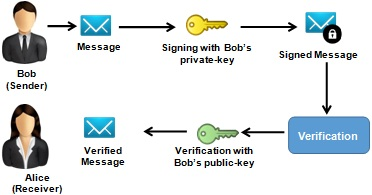
\includegraphics[scale=1.0]{images/AliceBob.jpg}
\caption{Signatures validated by public/private key.}
\label{fig:authenticationExample}
\end{center}
\end{figure}

\subsection{Consensus}\label{sec:consenso}
The key to blockchain operation is that the network must agree collectively on the ledger's content.  Instead of a central entity maintain control over information (such as a bank, for example), the data is shared among all. This requires the network to maintain the consensus around the information recorded in the blockchain. How this consensus is reached affects the security and economic parameters of the protocol \cite{kostarev2017review}.

In this context, consensus emerges as a fundamental problem since it allows distributed participants to coordinate their actions to reach joint decisions, ensuring the consistency of safety and system progress (liveness) despite failures \cite{greve2018blockchain}. More specifically, in the context of blockchain, consensus enables an agreement on the next block that will be added to the blockchain.

In the blockchain, reaching consensus between untrusted nodes is a transformation of the problem of \ac{BG} \cite{lamport1982byzantine}. In the BG problem, a group of generals who command a portion of the Byzantine army circles the city. The attack would fail if only part of the generals attacked the city. Generals need to communicate to agree on the attack or not. However, there may be traitors in the generals. The traitor could send different decisions to different generals. This is an environment without trust.

Reaching consensus in such an environment is a challenge. This is also a challenge for blockchain because its network is distributed, and there is no central node that ensures that ledgers on distributed nodes be all the same. Nodes do not need to trust other nodes. Thus, some protocols are required to ensure that ledgers on different nodes are consistent \cite{kostarev2017review}. To solve the consensus problem, several algorithms have been proposed and are listed below. For more details on each algorithm is recommended to read the article \cite{mingxiao2017review}.

\begin{itemize}
\item Proof-of-Work;
\item Proof-of-Stake;
\item Delegated Proof-of-Stake;
\item Leased Proof-Of-Stake;
\item Proof of Elapsed Time;
\item Practical Byzantine Fault Tolerance;
\item Simplified Byzantine Fault Tolerance;
\item Delegated Byzantine Fault Tolerance;
\item Directed Acyclic Graphs;
\item Proof-of-Activity;
\item Proof-of-Importance;
\item Proof-of-Capacity;
\item Proof-of-Burn;
\item Proof-of-Weight;
\end{itemize}

A good consensus algorithm means efficiency, security, and convenience. Current standard consensus algorithms still have many shortcomings. New consensus algorithms are created to solve some blockchain-specific problems \cite{zheng2016blockchain}.

\begin{figure}[htbp]
\begin{center}
  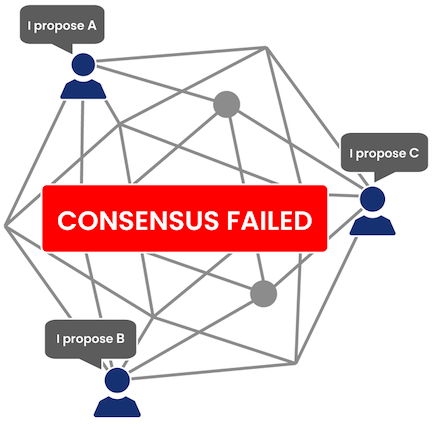
\includegraphics[scale=0.55]{images/consensus.png}
\caption{Consensus Mechanism}
\label{fig:Consensus}
\end{center}
\end{figure}


\subsection{Distributed Ledger}\label{sec:livro}
A distributed ledger is a data structure distributed by several nodes or computing devices. Each node replicates and saves an identical ledger copy. Each participating node in the network updates independently \cite{greve2018blockchain}.

The innovative feature of distributed accounting technology is that any central authority does not maintain the ledger. Updates to The ledger are independently constructed and recorded by each node. The nodes then vote on these updates to ensure that most agree on the conclusion, based on some previous consensus algorithm. Once consensus has been reached, the distributed ledger updates itself, and the latest agreed version is saved on each separate node \cite{swan2015blockchain}. Thus, the distributed ledger is replicated and immutable. 

\subsubsection{Transactions}\label{sec:transac}
The blockchain is a public digital book that records online transactions. In it, transactions are recorded in a block without the help of third parties, such as a bank or payment processor. The blockchain algorithm automatically graphs and authenticates the transaction, which is immediately visible to all users, minimizing the possibility of fraud. The terms of a transaction do not include any personal or identifying information \cite{Bankrate2018}.

The most fundamental definition of a transaction is an atomic event allowed by the underlying protocol from a technical standpoint. A transaction determines a sequence of state operations.  It adds a transfer of an asset or, generally speaking, a smart contract.  In a basic case, the transaction girds a digital signature of the issuer holding the asset and the receiver's address and inputs and outputs for the transaction. Each transaction must contain both Inputs and Outputs, just like in an accounting book. Entries indicate the previous transaction hash related to the current one \cite{greve2018blockchain}. Validating a Transition involves:

\begin{enumerate}
	\item signature verification;
	\item confirmation of existing values from hashes of previous referenced transactions;
	\item confirmation that any other transactions did not previously spend the amount.
\end{enumerate}

In this case, it is necessary to search the blockchain between the block from the referenced transaction to the last block of the structure. Each node of the blockchain network independently validates transactions, and this feature contributes to the decentralization of the process \cite{greve2018blockchain}.

\subsubsection{blocks}\label{sec:blocks}
Blocks contain a header with the information needed for the current maintenance and its validation. A block consists of the block header and block body, as shown in Figure \ref{fig:block}. 

\begin{figure}[htbp]
\begin{center}
  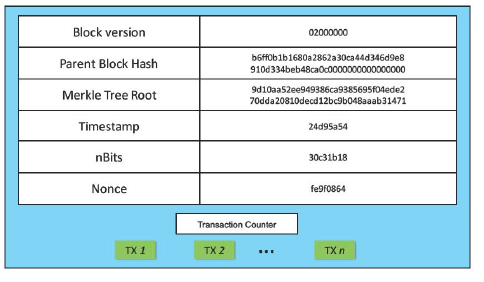
\includegraphics[scale=0.5]{images/blockStructure.png}
\caption{Structure of a block. \cite{zheng2016blockchain}}
\label{fig:block}
\end{center}
\end{figure}

In particular, the header Pack includes:

\begin{itemize}
\item Block version: indicates which set of block validation rules to follow.
\item Parent block hash: A 256-bit hash value that points to the previous block.
\item Merkle tree root hash: The hash value of all transactions in the block.
\item Timestamp: Current date and time as seconds since 1970-01-01T00:00 UTC.
\item  nBits: current hashing target in a compact format.
\item Nonce: A 4-byte field, usually starting with 0 and increasing for each hash.
\end{itemize}

The body's block consists of a transaction counter and transaction. The maximum number of transactions a block can hold depends on block size and the size of each transaction. Blockchain uses an asymmetric encryption mechanism to validate transaction authentication. A digital signature based on asymmetric encryption is used in an untrusted environment \cite{zheng2016blockchain}.

The validation of a block consists in verifying (i) if its structure is well-formed (ii) its hash is valid (meets the challenge), (iii) its size is within the network accepted limit, (iv) the set of transactions within the block is valid, (v) the first transaction (and only the first) is the coinbase transaction - which incorporates the generation of new cryptocurrencies in the system, besides acting as a reward mechanism. The blocks are validated independently by each node of the blockchain network, and this feature contributes to the process of decentralization \cite{greve2018blockchain}.

Figure \ref{fig:blockchain} presents a visual representation of a blockchain \cite{tian2017supply}.

\begin{figure}[htbp]
\begin{center}
  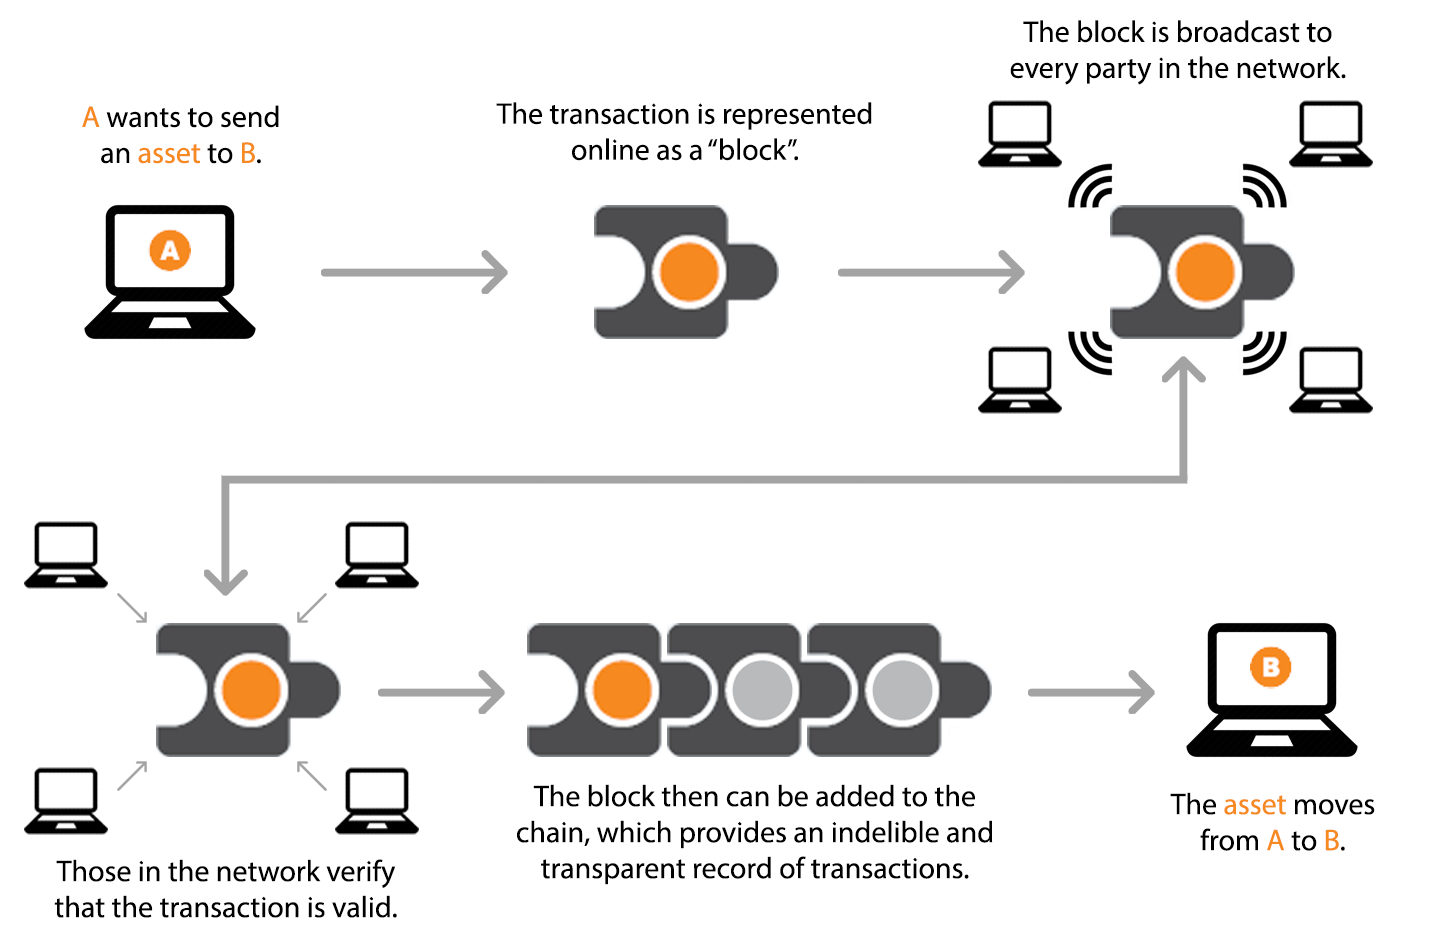
\includegraphics[scale=0.35]{images/blockchain.png}
\caption{Blockchain representation \cite{michael2018blockchain}}
\label{fig:blockchain}
\end{center}
\end{figure}

\section{Public Blockchain Versus Permissioned Blockchain}\label{sec:versus}

Blockchain networks can be categorized into two groups: public (or permissionless) blockchain and private (or federated or permissioned) blockchain (with permission and controlled access) \cite{greve2018blockchain}.

Since the beginning of blockchain technology, people have debated about public vs. permissioned blockchain. In an enterprise environment, it is essential to know the significant differences between these two. Public and permissioned blockchain examples play a considerable role in the companies looking for the perfect blockchain type for their solutions \cite{101blockchains}. Table \ref{table:pubVsPriv} presents a comparison between public and permissioned blockchain.

The primary difference between public and private blockchain is the level of access participants are granted. In order to pursue decentralization to the fullest extent, public blockchains are entirely open. Anyone can participate by adding or verifying data. The most common examples of public blockchain are Bitcoin (BTC) and Ethereum (ETH). These cryptocurrencies are created with open-source computing codes, which can be viewed and used by anyone. A public blockchain is about accessibility, which is evident in its use \cite{selfkeyOrg}. 

Conversely, permissioned blockchain (also known as private blockchain) only allows certain entities to participate in a closed network. Participants are granted specific rights and restrictions in the network, to have full access or limited access at the network's discretion. As a result, permissioned blockchain is more centralized as only a small group controls the network. The most common examples of permissioned blockchains are Ripple (XRP) and Hyperledger \cite{blockgeeks2018deeper}.

Additionally, some public blockchains also allow anonymity, while permissioned ones do not. For example, anyone can buy and sell Bitcoin without having their identity revealed. It allows everyone to be treated equally. Whereas with permissioned blockchains, the identities of the participants are known. This is typical because permissioned blockchain is used in the corporate and business-to-business sphere, where it is crucial to know who is involved \cite{101blockchains}.

\subsection{Public blockchain}\label{sec:blockchainPublica}
On a public or permissionless blockchain, any person can participate without a specific identity. There are no restrictions when it comes to participation. Public blockchains typically involve a native cryptocurrency and often use \acf{PoW} consensus and economic incentives \cite{androulaki2018hyperledger}. Anyone can audit public blockchain, and each node has as much transmission power as any other. For a transaction to be considered valid, it must be authorized by all nodes constituents via the consensus process. As long as each node meets protocol-specific stipulations, their transactions can be validated and thus added to the chain \cite{Comstor2018}.

In a public blockchain, all the participants have equal rights no matter what. People can join in and participate in consensus, transact with their peers as they please. Everyone can see the ledger as well, thus maintaining transparency at all times \cite{101blockchains}.

As the P2P network node-set is unknown, its membership is dynamic, allowing random node entrances, exits, and anonymity. Blockchain can act globally without the control of its participants, who do not even trust each other mutually. Are examples of public blockchain: the Bitcoin network, Ethereum, and several other cryptocurrencies \cite{bashir2018mastering, antonopoulos2017mastering}.

If a fully decentralized network system is required, then public blockchain is the way to go. However, it can get problematic when incorporating a public blockchain network with the enterprise blockchain process \cite{101blockchains}.

The main characteristics of a public blockchain are:

\begin{itemize}
\item High security: Public blockchain companies always design every single platform in a way that offers complete security.
\item Open environment: public blockchain is open for all. The system typically has an incentive mechanism to encourage more participants to join the network.
\item Anonymous nature: Everyone is anonymous. Users will not use their real name or real identity here. Everything would stay hidden, and no one can track data based on that.
\item No regulations: Public blockchain does not have any regulations that the nodes have to follow. So, there is no limit to how one can use this platform for their betterment. However, the main issue is that enterprises cannot work in a non-regulated environment.
\item True decentralization: public blockchain provides true decentralization. This is something that is quite absent in private blockchain networks. As everyone has a copy of the ledger, it creates a distributed nature as well. Basically, in this type of blockchain, there is not a centralized entity. Thus, the responsibility of maintaining the network is solely on the nodes. With help from a consensus algorithm, they are updating the ledger, promoting fairness.
\item Full transparency: Public blockchain companies tend to design the platforms fully transparent to anyone on the ledger. It means that users can see the ledger anytime they want. So, there is no scope for any corruption or discrepancies. Anyhow, everyone has to maintain the ledger and participate in consensus.
\item Immutability: The public blockchain network is fully immutable. Once a block gets on the chain, there is no way to change it or delete it. So, it ensures that no one can alter a particular block to benefit from others.
\end{itemize}

\subsubsection{Consensus for Public Blockchain}\label{sec:consensoPublica}
Due to the uncertainties regarding the participants, public blockchains generally adopt mining-based consensus mechanisms. In these mechanisms, miners vie with each other for consensus leadership, using computational power, possession power over cryptocurrency or other election-relevant powers that cannot be monopolized such that the same knots always come out victorious) \cite{greve2018blockchain}.

Compensation to these miners for their work is often cryptocurrency. These incentives are critical to preventing Byzantine attacks by solving the fundamental challenge of agreement globally. Currently, proof of work is one of the few prosperous and resilient consensuses approaches to Sybil attacks \cite{douceur2002sybil} (impersonation attacks, when malicious users become impersonate others).

In the mining process, new transactions are vilified by the nodes in the whole system known as “miners” before being added to the blockchain. Miners add new blocks on the chain or new transactions on the block by a consensus algorithm, which must be confirmed by the majority of all the nodes in the system, like a voting operation, as the valid data. Blockchain-based systems rely on miners to aggregate transactions into blocks and append them to the blockchain. Once a sufficient number of nodes confirms the transaction, it becomes a valid and permanent part of the database. 

\subsection{The pros and cons of public blockchain}\label{sec:prosConsPub}

One of the most significant advantages of a public blockchain is that there is no need for trust. Everything is recorded, public, and cannot be changed. Everyone is encouraged to do the right thing for the betterment of the network. There is no need for intermediaries \cite{blockgeeks2018deeper}.

The other significant advantage is security. The more decentralized and active a public blockchain is, the more secure it becomes. As more people work on the network, it becomes harder for any attack to succeed. It is nearly impossible for malicious actors to band together and control the network \cite{selfkeyOrg}.

The final piece of what makes public blockchain successful is transparency. All data related to transactions are open to the public for verification. The transparency of public blockchain increases potential use cases, such as decentralized identity \cite{Comstor2018}.

One of the biggest problems with public blockchain is speed. Public blockchains like Bitcoin are extremely slow, only managing to process seven transactions per second. Compare that to Visa, which can do 24,000 transactions per second, and we see where the problem is. Public blockchains are slow because it takes time for the network to reach a consensus. Additionally, the time needed to process a single block takes a long time compared to a private blockchain \cite{blockgeeks2018deeper}.

Public blockchains also face scalability concerns. With the current state of things, public blockchains cannot compete with traditional systems. The more a public blockchain is used, the slower it gets because more transactions clog the network. However, steps are being taken to remedy this problem. An example is Bitcoin’s Lightning Network \cite{selfkeyOrg}.

Lastly, energy consumption has been a concern when it comes to the public blockchain. Bitcoin’s algorithm relies on Proof-of-Work, which relies on using much electricity to function. That being said, other algorithms such as Proof-of-Stake use far less electricity \cite{selfkeyOrg}. 


\subsection{Permissioned Blockchain}\label{sec:blockchainPrivada}
Permissioned, federated, or private blockchains, on the other hand, perform a blockchain between a set of known and identified participants. A permissioned blockchain provides a way to protect the interactions between entities with a common goal but does not trust each other, like companies that trade funds, assets, or information. Relying on peer identities, one permissioned blockchain may use the traditional consensus of \acf{BFT} \cite{androulaki2018hyperledger}.

Federated blockchain has its known composition. It is formed by $n$ processes whose inputs and outputs are subject to permissions. Participants are identified, authenticated, and authorized. This blockchain model aims to serve better corporate or private interests where participants have well-defined roles and can even organize themselves into groups. Examples of permissioned blockchain are Hyperledger Fabric \cite{cachin2016architecture} and some other projects \cite{cachin2017blockchain}.

As enterprises need privacy, permissioned blockchain use cases seem a perfect fit in this case. Without proper privacy, their competition can enter the platforms and leaks valuable information to the press. This, in the long term, can influence the brand value greatly. So, in some instances, companies need privacy greatly \cite{101blockchains}.

The main characteristics of a public blockchain are:

\begin{itemize}
\item High efficiency: Compared with a public blockchain, which tends to lack inefficiency because it introduces everyone to the network. As a result, when more people try to use the features, it takes up many resources that the platforms cannot back up. Thus, it slows down rapidly. On the other hand, private blockchain only allows a handful of people in the network. In many cases, they even have specific tasks to complete. So, there is no way they can take up extra resources and slow down the platform.
\item Full privacy: Private blockchain tends to focus on privacy concerns. Enterprises always deal with security ad privacy issues. More so, they also deal with such sensitive information daily. If even one of them gets leaked, it can mean a massive loss for the company.
\item Empowering enterprises: Private blockchain solutions work to empower the enterprises as a whole rather than individual employees. In reality, companies do need great technology to back up their processes. More so, these solutions are mainly for the internal systems of an enterprise. This is one of the best use cases of the private blockchain.
\item Stability: Private blockchain solutions are stable. Basically, in every blockchain platform, users have to pay a certain fee to complete a transaction. However, the fee can increase significantly in public platforms due to the pressure of nodes requesting transactions. When there are too many transaction requests, it takes time to complete them. More so, as time increases, the fee increases drastically.
\item Low fees: In private blockchain platforms, the transaction fees are meager. Unlike public blockchain platforms, the transaction fee does not increase based on the number of requests. So, no matter how many people request a transaction, the fees will always stay low and accurate.
\item Saves money: In reality, private blockchain saves much money. Maintaining a private blockchain is relatively simple compared to public blockchains. Private blockchain platforms take up only a few resources.
\item No illegal activity: Private blockchain platforms have authentication processes before any user logs into the network. What this process does is filter any intruders trying to get into the system.
\item Regulations: For enterprise companies that have to follow many rules and regulations, private blockchain outlines all the rules, and the peer nodes have to follow them.
\end{itemize}

\subsubsection{Consensus for permissioned blockchain}\label{sec:consensoPrivada}
Since it is a controlled network with $n$ known participants and identified by the federation, classic \acf{BFT} protocols and deterministic Byzantine consensus can be adapted to the blockchain \cite{androulaki2018hyperledger}.

In addition, there is no need to use incentives to the agreement, as the federation of stakeholders can establish its financial model of remuneration. Incentives, however, may be used for other purposes but, different from the evidence-based consensus, they are not essential to consensus \cite{greve2018blockchain}.

In the \ac{BFT} literature, replication consistency is maintained by two principles:

\begin{itemize}
\item No mistake: Leaders are prevented from making mistakes, so only one possible proposal per leader per rating.
\item Proposal Security: A (higher-ranked) proposal can extend, but not modify, any lower-ranking compromised log prefix \cite{abraham2017blockchain}.
\end{itemize}

\subsection{The pros and cons of permissioned blockchain}\label{sec:prosConsPriv}

A significant advantage of permissioned blockchain is speed. Permissioned blockchains have far fewer participants, meaning it takes less time for the network to reach a consensus. As a result, more transactions can take place. Permissioned blockchains can process thousands of transactions per second. Comparing that to Bitcoin's seven transactions per second is a massive difference \cite{di17blockchain}.

Permissioned blockchains are also far more scalable. Since only a few nodes are authorized and responsible for managing data, the network can process more transactions. The decision-making process is much faster because it is centralized \cite{selfkeyOrg}.

However, the centralization of permissioned blockchain is one of its most significant disadvantages. Blockchain was built to avoid centralization and permissioned blockchain inherently becomes centralized due to its private network \cite{blockgeeks2018deeper}.

Trust is also a more significant issue when it comes to permissioned blockchain. The credibility of a permissioned blockchain network relies on the credibility of the authorized nodes. They need to be trustworthy as they are verifying and validating transactions. The validity of records also can’t be independently verified \cite{blockgeeks2018deeper}.

Security is another concern with permissioned blockchain. With fewer nodes, it is easier for malicious actors to gain control of the network. Unfortunately, a permissioned blockchain is far more at risk of being hacked or having data manipulated \cite{abraham2017blockchain}.

\begin{table}[H]
\caption{Public Vs. Permissioned blockchain \cite{101blockchains}:}
\label{table:pubVsPriv}
    \begin{tabular}{|l|p{5.61cm}|p{5.61cm}|}
        \hline 
        \thead{} & \thead{Public blockchain } & \thead{Permissioned blockchain}\\
        \hline 
        Access & Anyone & Single Organization\\
        \hline
        Authority & Decentralized & Partially decentralized\\
        \hline
        Transaction Speed & Slow & Fast\\
        \hline
        Consensus & Permissionless & Permissioned\\
        \hline
        Transaction Cost & High & Low\\
        \hline
        Data Handling & Read and Write access for anyone & Read and Write access for a single organization\\
        \hline
        Immutability & Full & Partial\\
        \hline
        Efficiency & Low & High\\
        \hline
    \end{tabular}
\end{table}

\section{Smart Contracts}\label{sec:smartContracts}

Blockchain 2.0 begins with the innovative proposal of smart contracts in 2013, and all range of possible financial applications \cite{greve2018blockchain}. A smart contract is a computerized transaction protocol that executes the terms of a contract \cite{szabo1997idea}. Its model was proposed a long time ago and now this concept can be implemented with blockchain.

The term \acf{SC} has been standardized by Nick Szabo in the 90s \cite{greve2018blockchain}. It means: “an internal transaction protocol format that executes the terms of a contract. Their overall goals are ensure common contractual conditions (such as payment terms, liens, confidentiality and even compliance), minimize malicious and accidental exceptions and the need for reliable intermediaries. Related economic objectives include reducing fraud losses, arbitration and execution costs, and other transaction costs.” \cite{szabo1997idea}.

Smart contract searches can be classified into two types: development and evaluation. Development can be development of smart contract or smart contract platform development. Recently, many smart contracts have been implemented on the Ethereum blockchain \cite{wood2018secure}. Regarding the platform development, many smart contracting platforms like Ethereum \cite{wood2018secure} and Hawk \cite{kosbaa2016theblockchain} are emerging \cite{zheng2016blockchain}. Evaluation means code analysis and performance evaluation. Errors in smart contracting can bring disastrous damage. Smart contract attack analysis is very important. On the other hand, smart contract performance is also vital to the contract. With the rapid development of blockchain technology, more and more smart contract based applications will be placed in use and companies need to consider performance of application \cite{zheng2016blockchain}.

In the blockchain, smart contracts are created as scripts, stored in with exclusive addressing on the blockchain itself \cite{greve2018blockchain}. They are triggered when addressing a transaction to it. Then the script is executed independently and automatically, as prescribed in all nodes in the network according to the data included in the transaction \cite{christidis2016blockchains}.

\subsection{Smart Contracts Security}\label{sec:seguranca}
Smart contracts interpret the code objectively - "The Code is the law". However, a code error was the target of cyber attack, resulting in a deviation of about \$50 million dollars, forcing Ethereum to perform a hard fork to perform a recovery \cite{bashir2018mastering}. Performing recoveries like this is not trivial, so the risks must be evaluated and minimized.

Smart contracts should be concerned with blockchain threats:
\begin{itemize}
\item State of contract.
\item Random generation.
\item Time Restrictions.
\end{itemize}

Regarding the status of the contract, field and balance values determines the smart contract state. A user when invoking it may not have certainty under its state, as other transactions may modify it or a fork may have occurred. In some cases, this can create vulnerabilities and lead to asset theft. In random generation, some contracts generate pseudo-random numbers with the same seed for all miners. This allows everyone to have the same view as Blockchain, providing
a malicious miner to influence the network. About time restriction, if a miner holds a stake in a contract, he can gain an advantage by choosing an appropriate time stamp for the block he is exploring \cite{greve2018blockchain}.
\section{Supply Chain Management and blockchain}\label{sec:scmBlock}

In order to solve some problems with Supply chain visibility and traceability, many internet of things technologies, such as RFID and wireless sensor network-based architectures and hardware, has been applied. However these technologies doesn't guarantee that the information shared by supply chain members in the traceability systems can be trusted. As a centralized organization, it can become a vulnerable target for bribery, and then the whole system can not be trusted anymore \cite{tian2017supply}.

Blockchain and distributed ledger technology underpinning cryptocurrencies such as Bitcoin, represent a new and innovative technological approach to realizing decentralized trustless systems. Indeed, the inherent properties of this digital technology provide fault-tolerance, immutability, transparency and full traceability of the stored transaction records, as well as coherent digital representations of physical assets and autonomous transaction executions \cite{caro2018blockchain}.

Blockchain enables end-to-end traceability, bringing a common technology language to the supply chain, while allowing consumers to access the assets history of these products through a web app. The need to track products across the complex supply chain from mineral prospecting and exploration to the end consumer is increasingly common: checking environmental impacts, or simply ensuring transparency for consumers \cite{galvez2018future}.


Instead of storing data in an shadowy network system, blockchain allow all the goods' information to be stored in a shared and transparent system for all the members along the supply chain \cite{tian2017supply}. Monfared \cite{abeyratne2016blockchain} argued about the potential benefit of blockchain technology in manufacturing supply chain. They proposed that the inherited characteristics of the blockchain enhance trust through transparency and traceability within any transaction of data, goods, and financial resources. And it could offer an innovative platform for new decentralized and transparent transaction mechanism in industries and business.

There are many members among the supply chain, including suppliers, producers, manufacturers, distributors, retailers, consumers and certifiers. Each of these members can add, update and check the information about the product on the blockchain as long as they register as a user in the system. Each product has also a unique digital cryptographic identifier that connects the physical items to their virtual identity in the system. This virtual identity can be seen as the product information profile. Users in the system also have their digital profile, which contains the information about their introduction, location, certifications, and association with products \cite{tian2017supply}.

Supply chain members can register themselves in the system as a user through the register, which can provide credentials and a unique identity to the members. After registration, a public and private cryptographic key pair will be generated for each user. The public key can be used to identify the identity of the user within the system and the private key can be used to authenticate the user when interacting with the system. This enables each product can be digitally addressed by the users when being updated, added, or exchanged to the next user in the downstream position of the supply chain. Administrator members are responsible for provide specific roles for each member/user \cite{caro2018blockchain}.

All members of the business network agree with the information acquired in each transaction. Once consensus is reached, no permanent record can be changed. Each information provides critical data that can potentially reveal security issues with the product in question \cite{galvez2018future}.

Smart contract encodes the combination of services and other conditions defined in the contract. Therefore, the smart contract can automatically verify and apply these conditions. It also verifies all information required by regulation to enable automated verification of regulatory compliance \cite{lu2017adaptable}. 

Smart contracts running on a blockchain can be accessed and called by all participants. A smart contract by default has no owner. Once deployed, its author has no special privileges. Unauthorized users may accidentally trigger a function without permission. Therefore, smart contracts must have an internal permission to verify contract permissions.

The smart contract structural design has a big cost impact if the blockchain is public. The cost of contract implementation depends on its size, because the code is stored in the blockchain, which implies data storage fees proportional to the size of the contract. Therefore, a structural design with more lines of code costs more. A blockchain consortium does not have coin or token, so the monetary cost is not a problem. However, blockchain size is still a design concern because it grows with each transaction and each participant has a replica of the entire blockchain. In addition, a more structural design may affect performance as it may require more transactions \cite{lu2017adaptable}.

Because blockchain technology is still at an early stage of development, there is a general lack of standards for implementation. A blockchain must be universal and adaptable to specific situations \cite{valenta2017comparison}. In addition, the need to agree on a particular type of blockchain to be used puts the parties under pressure. This is a major disadvantage as blockchain technology is progressing rapidly, and predicting the best choice for the future is quite difficult \cite{galvez2018future}.

On the other hand, there are advantages of applying the blockchain concept to the mineral supply chain. One of the most important is: all stakeholders involved in the supply chain (Raw material / Producer, Manufacturer, Distributor, Wholesaler, Retailer) are motivated by the need to demonstrate to customers the superior quality of their methods and products \cite{lu2017adaptable}. 

In addition to serving the functions of a traceability system, a blockchain can be used as a marketing tool. Because block chains are fully transparent\cite{iansiti2017truth} and participants can control the assets in them \cite{liao2011food}, they can be used to enhance image and reputation of a company \cite{van2007essentials}, drive loyalty among existing customers \cite{pizzuti2015global} and attract new ones \cite{svensson2009transparency}. 

In fact, companies can easily distinguish themselves from competitors by emphasizing transparency and monitoring product flow along the chain. In addition, quickly identifying a source of contamination or loss can help protect a company's brand image \cite{mejia2010traceability} and alleviate the adverse impact of media criticism \cite{dabbene2011food}.

\subsection{Transparency}\label{sec:transparency}

The main goals of a blockchain are to facilitate information exchange, create a digital twin of information and its workflow, and validate the quality of assets as they move along the chain. These goals are achieved by allowing each participant to share claims, evidence and assessments of each other's claims about the product. The journey of mineral resources along the supply chain is captured in a blockchain object called a "mineral bundle". At the end of the journey, the package is the combination of all information provided by stakeholders over the life of the mineral item. This information can be used to establish the provenance, quality, sustainability and many other attributes of mineral assets \cite{martin2017technology}.

\subsection{Efficiency}\label{sec:efficiency}
Blockchain is an infrastructure that allows new transactions between players who do not yet know or trust each other. Smart contracts are instructions that interface with the blockchain protocol to automatically evaluate and possibly post transactions on the blockchain \cite{raskin2017law}. 

Similarly, smart libraries are specialized sets of blockchain-compatible functionality that can be used locally or privately or shared and licensed to other blockchain participants and agents. All participants meet at the blockchain, can evaluate the statements made and notify their account holders when matches are found in quality, time, quantity, etc. Buyers and sellers are matched by a shared but reliable need for data that can be combined and used by either party. So traceability doesn't have to wait for large company consortia to use patterns and / or semi-mandatory or concentrated business practices to access the information \cite{galvez2018future}.

\subsection{Safety and protection}\label{sec:Safety}
Blockchains can also be used to emit and manage the creation of unique cryptographic tokens \cite{nystrom1999pkcs}. Tokens can be made to represent the collateral value between two participants (for example, future production to be sent in a specific field lot). In fact, tokens do not have to take the form of value exchange for financial settlement of invoices and contracts. Instead, they represent a license to publish information that becomes uniquely valued in proportion to the needs of others on the blockchain. The strategy around issuing these encryption tokens, which need not be implemented in the initial system, is still being defined \cite{galvez2018future}.
\section{Hyperledger Fabric}\label{sec:hyperledger}

As the popularity of public blockchain and a few other derivative technologies grew, interest in applying the underlying technology of the blockchain, distributed ledger, and distributed application platform to more innovative enterprise use cases also grew. However, many enterprise use cases require performance characteristics that permissionless blockchain technologies are unable (presently) to deliver. In addition, in many use cases, the identity of the participants is a hard requirement, such as in the case of financial transactions where Know-Your-Customer (KYC) and Anti-Money Laundering (AML) regulations must be followed \cite{POLGE2020}.

For enterprise use, it is necessary to consider the following requirements:

\begin{itemize}
\item Participants must be identified/identifiable;
\item Networks need to be permissioned;
\item High transaction throughput performance;
\item Low latency of transaction confirmation;
\item Privacy and confidentiality of transactions and data of business transactions.
\end{itemize}

These requirements are a good fit with the required non-functional requirements for an SCM project and the ones specified in table~\ref{table:rnf}. While many early blockchain platforms are currently being adapted for enterprise use, Hyperledger Fabric has been designed for enterprise use from the outset. 

The Hyperledger Project is a collaborative effort to create an enterprise-grade, open-source distributed ledger framework, and codebase. It aims to advance blockchain technology by identifying and realizing a cross-industry open standard platform for distributed ledgers, transforming how business transactions are conducted globally \cite{cachin2016architecture}.

Hyperledger Fabric implements a distributed ledger platform for running smart contracts, leveraging familiar and proven technologies, with a modular architecture allowing pluggable implementations of various functions \cite{cachin2016architecture}. Hyperledger Fabric is a widely used permissioned blockchain-primarily in enterprise settings to make transactions between multiple businesses more efficient. This implementation defines assets and the transaction instructions. Members of each permissioned network interact with the ledger using chaincode. The Membership identity service manages IDs and authenticates participants. Also, the Access Control List provides additional layers of permission \cite{blockgeeks2018deeper}.

\begin{figure}[htbp]
\begin{center}
  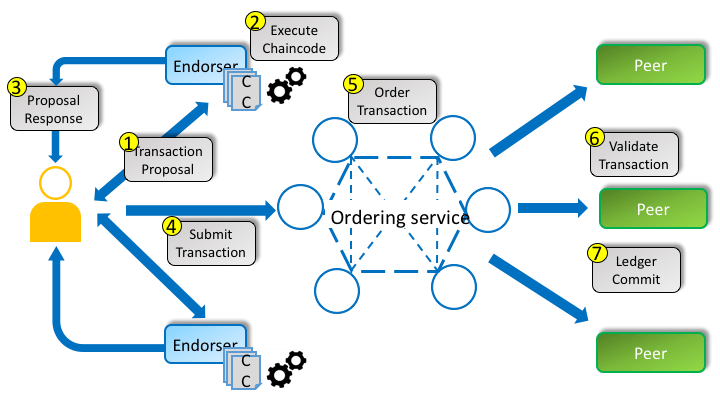
\includegraphics[scale=0.43]{images/Hyperledger-Fabric-high-level-transaction-flow.png}
\caption{Hyperledger Fabric  transaction flow \cite{manevich2018service}.}
\label{fig:hyperledgerFlow}
\end{center}
\end{figure}

There are two types of nodes in Hyperledger Fabric: peer nodes and ordering nodes. Peer nodes are responsible for executing and verifying transactions while ordering nodes are responsible for ordering transactions and propagating the correct history of events to the network. This increases efficiency and scalability by allowing peer nodes to batch and process multiple transactions \cite{buterin2016smart}. 

Fabric Ledger comprises two components: A blockchain log to stores the immutable sequenced record of transactions in blocks and a State Database to maintain the blockchain's current state. In a public blockchain, there is no state database. It means that the chain's current state is always calculated by going through all the transactions in the ledger. For speed and efficiency, the Fabric stores the current state and allows network members to query it as a SQL-like transaction \cite{blockgeeks2016blockchain}. 

Figure~\ref{fig:hyperledgerFlow} shows the Hyperledger Fabric transaction flow. The client proposes a transaction to the endorsing peers  and collects transaction responses. The client then submits a transaction to the ordering service, which orders incoming transactions and cuts them into blocks. Peers pull blocks from the ordering service, validate the transactions, append them to the ledger, and apply valid transactions to the state.

The log aims to trap an asset providence or place of origin as it exchanges among multiple parties. To track an asset's provenance means to track where and when it was created, and every time it was exchanged. Tracking an asset's providence is extremely important in business because it ensures that the business selling an item possesses a chain of titles verifying their ownership of it. In typical databases, where only the current state is kept and not a log of all transactions, tracking an asset providence becomes very difficult. Add to this the fact that transacting businesses each keep an incomplete record of the asset transaction, and it becomes nearly impossible \cite{blockgeeks2016blockchain}.

Fabric uses Private Channels to solve the problem of sensitive data which other parties or competitors could see in a public blockchain. Private Channels are restricted message paths that can provide transaction privacy and confidentiality for a specific subset of network members. All data are invisible and inaccessible to any network members not explicitly granted access to that channel. This allows competing business interests and any groups that require private, confidential transactions to coexist on the same permissions network \cite{brabbani2017hashing}.

\xchapter{Related Work}{This section presents some orthodox and blockchain based SCM systems, their main characteristcs and how this work presents a new approach different from them.}\label{chap:RelatedWork}

% É recomendável utilizar `\acresetall' no início de cada capítulo para reiníciar o contator de referências às siglas.
\acresetall 

The rapid growth of internet technologies allowed the onset of lots of technologies applied in traceability systems. In order to solve some problems with Supply Chain traceability, many Internet of Things (IoT) technologies, such as RFID and wireless sensor network-based architectures have been applied. However, these technologies do not guarantee that the information shared by supply chain members in the traceability systems can be trusted \cite{tian2017supply}.

Blockchain presents a whole new approach based on decentralization. Nonetheless, by being in its early stages, it has some challenges to deal with, in which scalability and performance become mainly defiance to face the massive amount of data in the real world. Through this technology, some solutions have been raised, as follows.

\section{Traditional Systems} \label{sec:TraditionalSystems}

Microsoft's Dynamics 365 is excellent for simple SCM needs, and it's just as accessible as every other Microsoft suite on the market. Dynamics integrates with third-party management systems, but it's primarily for "simple needs." Microsoft's offering isn't so great for complex supply chain demands - but then, the greater majority of organisations haven't got overly complex networks \cite{bellu2018microsoft}.

Plex Systems was one of the very first supply chain and manufacturing Software-as-a-Service (SaaS) ERP systems. The software is a cloud-based SCM that is very popular with industry-leading companies - especially in the aerospace and automotive industries. Unfortunately, though, for all its maturity and complex capabilities, Plex lets organisations down with its inability to support several implementation partners \cite{plex}.

Oracle NetSuite is a cloud based supply chain and ERP system for the less complex needs of companies moderately sized companies and the majority of SCM and ERP systems \cite{rolling2016using}. As ERP focused system, this project is focused on business management instead of SCM traceability and information transparency \cite{rolling2016using}.

SAP Supply Chain Management harnesses technologies such as AI and the Internet of Things to provide visibility and  analytics to help the users in planning, sourcing, and delivering the goods and materials.  This is a real-time supply chain planning software which connects stakeholders \cite{snapp2010discover}.

These systems typically are ERP solutions focused on business management, controlled by service providers.  This centralized data  storage becomes a single point of failure and risks tampering. As a centralized organization, it can become a vulnerable target for  bribery, and then the whole system can not be trusted anymore. Also as proprietary systems, there are some concerns about reliability, security, decentralization, immutability, transparency and lack of trust among participants as there is no trusted third party to ensure data reliability. 

\section{Blockchain based Systems} \label{sec:BlockchainBasedSystems}

There are advantages of applying the Blockchain concept to a supply chain. One of the most important is: all stakeholders involved in the supply chain are motivated by the need to demonstrate to customers the superior quality of their methods and products \cite{lu2017adaptable}. In addition, a Blockchain can be used as a marketing tool. As Blockchains are fully transparent and participants can control the assets in them, they can be used to enhance image and reputation of a company \cite{van2007essentials}, drive loyalty among existing customers \cite{pizzuti2015global} and attract new ones \cite{svensson2009transparency}. In fact, companies can easily distinguish themselves from competitors by emphasizing transparency and monitoring product flow along the chain. 

In \cite{tian2017supply}, it is proposed a system that combines HACCP (a food safety protocol), Blockchain and IoT in order to provide food safety traceability. Each member can add, update and check the information about the product on the Blockchain as long as they register as a user in the system. Each product also has a unique digital cryptographic identifier that connects the physical items to their virtual identity in the system. This virtual identity can be seen as a product information profile.

The Everledger Diamonds project provides a Blockchain-based solution to facilitate tracking from mine to consumer, enabling easier compliance against increasingly strict measures from diamonds produced \cite{crosby2016blockchain}.

IBM Food Trust is a pilot project motivated by food contamination scandals worldwide. The main goal is to tackling food safety in the supply chain using Blockchain technology. This platform tracked pork in China and mangoes in the Americas \cite{kamath2018food}.

These projects are focused on specific products only and are closed projects. Still, there is a general lack of standards for implementation of a Blockchain approach for traceability. A Blockchain must be universal and adaptable to specific situations \cite{valenta2017comparison}. In addition, the need to agree on a particular type of Blockchain to be used puts the parties under pressure. 

Our work is intended to provide a Blockchain-based platform in order to facilitate the development of applications for traceability in supply chain management.
%\xchapter{General Context}{} %sem preambulo
\acresetall

Traceability systems typically store information in standard databases controlled by service providers. This centralized data storage becomes a single point of failure and risks tampering. As consequence, these systems results in trust problem, such as fraud, corruption, tampering and falsifying information. Likewise, by being a single point of failure, centralized system is vulnerable to collapse \cite{tian2017supply}.

Nowadays, a new technology called the blockchain presents a whole new approach based on decentralization. Blockchain enables end-to-end traceability, bringing a common technology language to the supply chain, while allowing consumers to access the assets history of these products through a software application \cite{galvez2018future}.

\section{Supply Chain Management and blockchain}\label{sec:scm}

The complex web of relationships that provide materials manufacture the components, assemble or mix the parts and deliver the final product to market is known as the supply chain \cite{buurman2002supply}.

In order to solve some problems with Supply chain visibility and traceability, many internet of things technologies, such as RFID and wireless sensor network-based architectures and hardware, has been applied. However these technologies doesn't guarantee that the information shared by supply chain members in the traceability systems can be trusted. As a centralized organization, it can become a vulnerable target for bribery, and then the whole system can not be trusted anymore \cite{tian2017supply}.

Blockchain and distributed ledger technology underpinning cryptocurrencies such as Bitcoin, represent a new and innovative technological approach to realizing decentralized trustless systems. Indeed, the inherent properties of this digital technology provide fault-tolerance, immutability, transparency and full traceability of the stored transaction records, as well as coherent digital representations of physical assets and autonomous transaction executions \cite{caro2018blockchain}.

Blockchain enables end-to-end traceability, bringing a common technology language to the supply chain, while allowing consumers to access the assets history of these products through a web app. The need to track products across the complex supply chain from mineral prospecting and exploration to the end consumer is increasingly common: checking environmental impacts, or simply ensuring transparency for consumers \cite{galvez2018future}.

When applied to the supply chain, digital product information such as prospecting source details, batch numbers, mining and processing data, storage and transportation details are digitally connected to mineral items and their information is entered into the blockchain at each step of the process \cite{caro2018blockchain}.

Instead of storing data in an shadowy network system, blockchain allow all the goods' information to be stored in a shared and transparent system for all the members along the supply chain \cite{tian2017supply}. Monfared \cite{abeyratne2016blockchain} argued about the potential benefit of blockchain technology in manufacturing supply chain. They proposed that the inherited characteristics of the blockchain enhance trust through transparency and traceability within any transaction of data, goods, and financial resources. And it could offer an innovative platform for new decentralized and transparent transaction mechanism in industries and business.

There are many members among the supply chain, including suppliers, producers, manufacturers, distributors, retailers, consumers and certifiers. Each of these members can add, update and check the information about the product on the blockchain as long as they register as a user in the system. Each product has also a unique digital cryptographic identifier that connects the physical items to their virtual identity in the system. This virtual identity can be seen as the product information profile. Users in the system also have their digital profile, which contains the information about their introduction, location, certifications, and association with products \cite{tian2017supply}.

Supply chain members can register themselves in the system as a user through the register, which can provide credentials and a unique identity to the members. After registration, a public and private cryptographic key pair will be generated for each user. The public key can be used to identify the identity of the user within the system and the private key can be used to authenticate the user when interacting with the system. This enables each product can be digitally addressed by the users when being updated, added, or exchanged to the next user in the downstream position of the supply chain. Administrator members are responsible for provide specific roles for each member/user \cite{caro2018blockchain}.

All members of the business network agree with the information acquired in each transaction. Once consensus is reached, no permanent record can be changed. Each information provides critical data that can potentially reveal security issues with the product in question \cite{galvez2018future}.

Smart contract encodes the combination of services and other conditions defined in the contract. Therefore, the smart contract can automatically verify and apply these conditions. It also verifies all information required by regulation to enable automated verification of regulatory compliance \cite{lu2017adaptable}. 

Smart contracts running on a blockchain can be accessed and called by all participants. A smart contract by default has no owner. Once deployed, its author has no special privileges. Unauthorized users may accidentally trigger a function without permission. Therefore, smart contracts must have an internal permission to verify contract permissions.

The smart contract structural design has a big cost impact if the blockchain is public. The cost of contract implementation depends on its size, because the code is stored in the blockchain, which implies data storage fees proportional to the size of the contract. Therefore, a structural design with more lines of code costs more. A blockchain consortium does not have coin or token, so the monetary cost is not a problem. However, blockchain size is still a design concern because it grows with each transaction and each participant has a replica of the entire blockchain. In addition, a more structural design may affect performance as it may require more transactions \cite{lu2017adaptable}.

Because blockchain technology is still at an early stage of development, there is a general lack of standards for implementation. A blockchain must be universal and adaptable to specific situations \cite{valenta2017comparison}. In addition, the need to agree on a particular type of blockchain to be used puts the parties under pressure. This is a major disadvantage as blockchain technology is progressing rapidly, and predicting the best choice for the future is quite difficult \cite{galvez2018future}.

On the other hand, there are advantages of applying the blockchain concept to the mineral supply chain. One of the most important is: all stakeholders involved in the supply chain (Raw material / Producer, Manufacturer, Distributor, Wholesaler, Retailer) are motivated by the need to demonstrate to customers the superior quality of their methods and products \cite{lu2017adaptable}. 

In addition to serving the functions of a traceability system, a blockchain can be used as a marketing tool. Because block chains are fully transparent\cite{iansiti2017truth} and participants can control the assets in them \cite{liao2011food}, they can be used to enhance image and reputation of a company \cite{van2007essentials}, drive loyalty among existing customers \cite{pizzuti2015global} and attract new ones \cite{svensson2009transparency}. 

In fact, companies can easily distinguish themselves from competitors by emphasizing transparency and monitoring product flow along the chain. In addition, quickly identifying a source of contamination or loss can help protect a company's brand image \cite{mejia2010traceability} and alleviate the adverse impact of media criticism \cite{dabbene2011food}.

Blockchain simplifies this challenging task by providing one-to-many data integration and process orchestration among participants. In addition, it provides a lexicon and ontology to describe asset attributes across the supply chain. This in turn facilitates the establishment of a data structure that can be used by smart contracts to automate claims, certifications and market operations. There are three elements to explain why the food supply chain can benefit from the blockchain concept, namely: transparency, efficiency, safety and security \cite{galvez2018future}.

\subsection{Transparency}\label{sec:transparency}

The main goals of a blockchain are to facilitate information exchange, create a digital twin of information and its workflow, and validate the quality of assets as they move along the chain. These goals are achieved by allowing each participant to share claims, evidence and assessments of each other's claims about the product. The journey of mineral resources along the supply chain is captured in a blockchain object called a "mineral bundle". At the end of the journey, the package is the combination of all information provided by stakeholders over the life of the mineral item. This information can be used to establish the provenance, quality, sustainability and many other attributes of mineral assets \cite{martin2017technology}.

\subsection{Efficiency}\label{sec:efficiency}
Blockchain is an infrastructure that allows new transactions between players who do not yet know or trust each other. Smart contracts are instructions that interface with the blockchain protocol to automatically evaluate and possibly post transactions on the blockchain \cite{raskin2017law}. 

Similarly, smart libraries are specialized sets of blockchain-compatible functionality that can be used locally or privately or shared and licensed to other blockchain participants and agents. All participants meet at the blockchain, can evaluate the statements made and notify their account holders when matches are found in quality, time, quantity, etc. Buyers and sellers are matched by a shared but reliable need for data that can be combined and used by either party. So traceability doesn't have to wait for large company consortia to use patterns and / or semi-mandatory or concentrated business practices to access the information \cite{galvez2018future}.

\subsection{Safety and protection}\label{sec:Safety}
Blockchains can also be used to emit and manage the creation of unique cryptographic tokens \cite{nystrom1999pkcs}. Tokens can be made to represent the collateral value between two participants (for example, future production to be sent in a specific field lot). In fact, tokens do not have to take the form of value exchange for financial settlement of invoices and contracts. Instead, they represent a license to publish information that becomes uniquely valued in proportion to the needs of others on the blockchain. The strategy around issuing these encryption tokens, which need not be implemented in the initial system, is still being defined \cite{galvez2018future}.

\section{Supply chain and mineral resources}\label{sec:scmMineral}

To begin with, the starting point of a supply chain is the extraction of raw materials and how they are first processed (preprocessed) by suppliers for delivery in the next step. The next step is called manufacturing, where the conversion process for raw materials takes place. Following this, the constructed products are passed to the distributors who are responsible for allocating them to multiple different intermediaries, such as wholesalers and retailers. Distributors also maintain an active inventory of products, as previous products are connected to suppliers. Subsequently, wholesalers do not sell products directly to the public, but to other retailers, whereas retailers dispose products purchased to end users. Finally, Consumers are who buy or receive goods or services for personal needs or use and not for commercial resale or trade purposes \cite{litke2019blockchains}.

The manufacturer can validate crucial information about the natural resources they collected by reading and verifying all tags that the latter includes in its transactions and then proceeding to the proper execution of manufacturing step. New transactions with new information tags, such as manufacturer name, field experience and more, are sent after the internship has completed. Then the products are delivered to distributors. Distributors are able to sell products to wholesalers and retailers. This process is represented by blockchain transactions that display important data tags, such as merchant and customer address, exchange value, product raw material quality, and more \cite{sauer2018extending}. 

As the distributors sell products to intermediates (generally not end users), they can check valuable tag information about the progress route until that stage, for example the raw material origin, manufactures company popularity, distributor address and others. Retailers can audit product's natural resource quality, and get the appropriate feedback before selling it to the consumer. After that, when a distributor send the product to the wholesaler by submitting a corresponding transaction, the latter tags, such as manufacturer name, field experience and others, are submitted after the completion of acts in a similar way. Wholesaler can check transaction data and execute their selling to another wholesaler or retailer company by submitting a new transaction. The same applies to the retailer companies. Finally, end users obtain the final product with a submitted transaction and is able to track and verify all aspects from the beginning of its supply chain journey \cite{litke2019blockchains}. 

\subsection{Exploration}\label{sec:Exploration}
Exploration is the starting point of a supply chain. Phase which encompasses Mineral Prospecting and Geological Survey.

\subsubsection{Prospecting/ Surveying}\label{sec:Prospecting}
Prospecting means the search of mineral occurrences/surveying means the research on a mineralised area, previously defined during the prospecting phase to be applied as a Mineral Right from the Mining Authority.

\subsubsection{Mining right application}\label{sec:Mining}
Through handing over documents to the Mining Authority (in Brazil it is \textit{Agência Nacional de Mineração} [ANM]).

\subsubsection{Geological Survey}\label{sec:GeologicalSurvey}
Geological Survey is a set of activities carried out to determine the features on quality and quantity of ore found in a given mineral deposit.

\subsubsection{Mineral reserve definition}\label{sec:MineralReserve}
this step is related to the quantity of ore found during the Geological Survey.

\subsection{Mine Development and Design}\label{sec:MineDevelopment}
In this phase is made the preparation of a deposit to become a mine, opening accesses, setting up fences, building benches.

\subsection{Production}\label{sec:Production}
Production phase including ore extraction and mineral processing or transformation.

\subsubsection{Quarrying/ Blasting plan}\label{sec:Quarrying}
Quantity of stone extracted, same quantity of mineral reserves depleted, type of stone extracted.

\subsubsection{Processing}\label{sec:Processing}
Quantity of stone crushed/processed, same quantity of stone in stock deducted, type of stone product, market requirements.

\subsubsection{Aggregate Product}\label{sec:AggregateProduct}
Listing of products with identified quantities and respective technological features.

\subsection{Distribution}\label{sec:Distribution}
Product distribution with identification of clients and their segmentation. 

\subsubsection{Client by Product Type}\label{sec:Client}
Name, address, size, sector, business registration numbers (federal, state, municipal, county).

\subsubsection{Transport}\label{sec:Transport}
Invoice, bills, type of transportation, weight, distance.

\subsection{Mine Closure}\label{sec:MineClosure}
Mine Closure or mineral decommissioning, it means the end of the mining activity and the start of the installations removal and area remodelling through plantation and/or building a lake.

\subsubsection{Legal Compliance/Decommissioning Plan}\label{sec:LegalCompliance}
Status of all documentation related to the Decommissioning Plan and its Legal Compliance.

\subsubsection{Environmental Recovery/ ANM Application}\label{sec:EnvironmentalRecovery}
Application number and status.


\xchapter{Technical Specification}{} %sem preambulo
\label{chap:Technical}

\acresetall 

\ac{SCM-BP} has the general objective to create a generic framework intended to be used in any kind of supply chain correlated to assets and products. Craton-Roche SCM-BP is a use case of this framework applied, initially, to the mining supply chain and more specifically, to the gravel ecosystem. The project is subdivided into the following specific objectives:
\begin{itemize}
\item Perform a survey of functional requirements.
\item Design system architecture.
\item Develop web application.
\item Develop smart contract.
\item Perform system validations.
\end{itemize}


\section{Application Architecture}\label{sec:applicationArchitecture}

\ac{SCM-BP} is divided into three main modules described below: WebApp - FrondEnd, WebApp - BackEnd and Data Storage. Figure~\ref{fig:detalhamentotecnico} shows the application architecture and its components. Figure~\ref{fig:dataStructure} present the main data structure.

\begin{figure}[htbp]
\begin{center}
  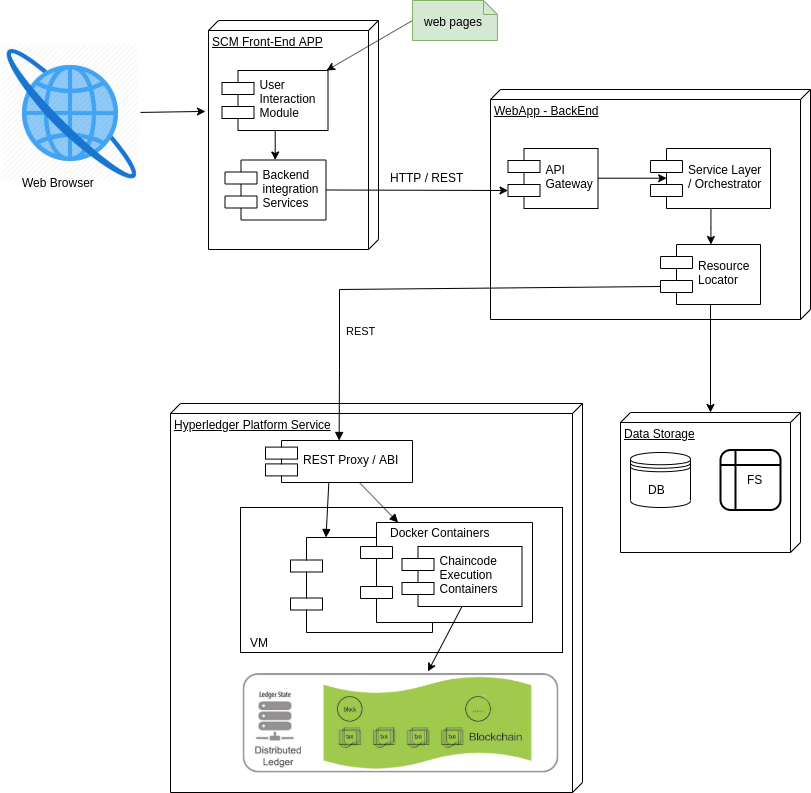
\includegraphics[scale=0.55]{images/detalhamentotecnico.png}
\caption{Application architecture of \ac{SCM-BP}}
\label{fig:detalhamentotecnico}
\end{center}
\end{figure}

\subsection{WebApp - FrondEnd}\label{sec:WebAppFrondEnd}
WebApp - FrontEnd is a client–server computer application which the client (including the user interface and client-side logic) runs in a web browser. This is a single-page application (SPA), a web application that interacts with the user by dynamically rewriting the current page rather than loading entire new pages from a server. This approach avoids interruption of the user experience between successive pages, making the application behave more like a desktop application.

The application is build with React (also known as React.js or ReactJS). This is a JavaScript library for building user interfaces. It is maintained by Facebook and a community of individual developers and companies. Used as a base in the development of single-page or mobile applications, React is optimal for fetching rapidly changing data that needs to be recorded. However, fetching data is only the beginning of what happens on a web page, which is why complex React applications usually require the use of additional libraries for state management, routing, and interaction with an API.

The Webapp - FrontEnd is divided into two main blocks and these are classified according to the interactions: User Interaction Modules and Backend Interactions Services.

\subsubsection{User Interaction}\label{sec:UserInteraction}
The User Interaction modules are responsible for providing web pages that will be rendered on client’s web browser. These interactions are provided by web pages grouped by the following modules:

\begin{itemize}
\item Login page
\item Application configuration module
\item User handling module (actors - CRUD)
\item Data entry module (forms)
\item Data visualization module
\item Reporting module
\end{itemize}

\subsubsubsection{Login Module}
The Login Module is responsible for display the login and authentication alternatives pages (‘forgot my password’, ‘reset my password’, etc.).

\subsubsubsection{Application configuration module}
The Application configuration module provides the features of creation/configuration of supply chain items and supply chain flows (steps and sub-tasks).

\subsubsubsection{User handling module}
This module provides the features for creation/configuration of Actors and Roles. The table in appendix \ref{app:userCreationFields} show the fields and values for creating a user.

\subsubsubsection{Data entry module}
The Data entry module provides form pages that allow users to enter data in the application, search and move assets from a step to another.

\subsubsubsection{Data visualization module}
The Data visualization module is responsible to display the information about assets in the supply chain flow. 

\subsubsubsection{Reporting Module}
In the Reporting module users can generate reports/files containing information organized in a narrative, graphic, or tabular form, prepared on ad hoc, periodic, recurring, regular, or as required basis. Reports may refer to specific periods, events, occurrences, or subjects, and may be presented in written form or any other format.

\subsubsection{Backend Interaction}\label{sec:BackendInteraction}
Backend interactions happen via a service layer consisting of:

\begin{itemize}
\item Authentication service
\item Application setup service
\item User creation service (actors)
\item Data entry service (forms)
\item Data visualization service
\item Reporting service
\end{itemize}

\subsubsubsection{Authentication Service}
The function of the Authentication Service is to request information from an authenticating party, and validate it against the configured identity repository using the specified authentication module. After successful authentication, the user session is activated and can be validated across all web applications participating in an SSO environment. For example, when a user or application attempts to access a protected resource, credentials are requested by one (or more) authentication modules. Gaining access to the resource requires that the user or application be allowed based on the submitted credentials.

\subsubsubsection{Application setup Service}
Application setup service provides methods to configure and edit  supply chain items and supply chain flows, defining which steps and sub-tasks will be present in this flow and which information will be present in these steps.

\subsubsubsection{User creation Service}
This service is responsible for the creation of users and roles, to allow them to log in and use the application’s features. Only Administrators are allowed to create new users (see Actions and Actors).

\subsubsubsection{Data entry Service}
Data entry service receives data from UI forms and send them to the backend to be processed and stored.

\subsubsubsection{Data visualization Service}
Data visualization services provides information about the supply chain: Assets, users and transactions, to be used by the data visualization module.

\subsubsubsection{Reporting Service}
Report services generate files (Doc/PDF/XSL, etc...) from a specific period of time with information about the supply chain: Assets, users and transactions.
\subsection{WebApp - BackEnd}\label{sec:WebAppBackEnd}
WebApp - BackEnd is a Middleware that runs on the server. This Middleware (server-side software) facilitates client-server connectivity, forming a middle layer between the app(s) and the network: the server, the database, the operating system, and more. It receives requests from the clients (in this case, the WebApp - FrontEnd), and contains the logic to send the appropriate data back to the applicant, over HTTP and REST.  These are the main conventions that provide structure to the request-response cycle between clients and servers.

WebApp - BackEnd is an application build with Node.js, an application platform where developers can write Javascript programs that are compiled, optimized and interpreted by the V8 virtual machine. Node.js can create quick, reliable websites and products in much efficient manner. Developing easy to scale real time applications in other technologies is bit difficult, but JavaScript technologies made it easier.

The WebApp - BackEnd is composed by the API Gateway, Service Layer and Resource Locator more detailed below.

\subsubsection{API Gateway}\label{sec:APIGateway}
API Gateway is a managed service that enables easily create, publish, maintain, monitor and secure REST APIs to act as a "gateway" for applications to access data, business logic, or functionality in the backend services, such as workloads. The API Gateway provides a simple uniform view of external resources to the internals of this application. It manages all tasks involved in receiving and processing API calls, including traffic management, authorization and access control, monitoring and management of API versions.

\begin{figure}[htbp]
\begin{center}
  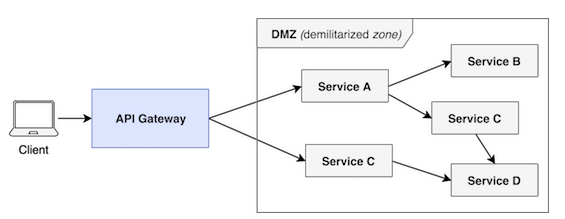
\includegraphics[scale=0.75]{images/apigateway.png}
\caption{API Gateway.}
\label{default-regular2}
\end{center}
\end{figure}

Basically, the Gateway is an interface that receives calls to its internal systems, being a large gateway. It act in five different ways:

\begin{itemize}
\item Filter for call traffic from different media;
\item Single gateway to the various APIs that are exposed;
\item Router: API and Rate Limit traffic router;
\item Security engine with authentication and logging.
\end{itemize}

Gateway access can be done from many different devices. Therefore, it must have the power to unify outgoing calls and be able to deliver to the user content that can be accessed from any browser and system. In this project the gateway interaction happens with the frontend webapp. The Gateways as a Security Feature: In the APIs world, one of the most subject talked about issues is always security, and having an API Gateway is one of the best solutions on the market to get full control of API’s, because this pattern addresses the so-called CIA (Confidentiality, Integrity, Availability) almost flawlessly.

\subsubsection{Service Layer}\label{sec:ServiceLayer}
A Service Layer defines an application's boundary and its set of available operations from the perspective of interfacing client layers. It encapsulates the application's business logic, controlling transactions and coordinating responses in the implementation of its operations.

Enterprise applications typically require different kinds of interfaces to the data they store and the logic they implement: data loaders, user interfaces, integration gateways, and others. Despite their different purposes, these interfaces often need common interactions with the application to access and manipulate its data and invoke its business logic. The interactions may be complex, involving transactions across multiple resources and the coordination of several responses to an action. Encoding the logic of the interactions separately in each interface causes a lot of duplication. the service layer provides:

\begin{enumerate}
\item Centralizes external access to data and functions.
\item Hides (abstracts) internal implementation and changes.
\item Allows for versioning of the services.
\end{enumerate}

The service layer acts as an orchestrator, controlling the flow of incoming and outcoming information requests and responses. Orchestration allows to directly link process logic to service interaction within workflow logic. This combines business process modeling with service-oriented modeling and design, realizing workflow management through a process service model. Orchestration brings the business process into the service layer, positioning it as a master composition controller.

\subsubsection{Resource Locator}\label{sec:ResourceLocator}

Resource locators are components that abstracts the persistence layer. Their job is to provide an object that can help services to discover and persist information from/to the Data Storage Module. Information can be stored in the Blockchain, Filesystem or Database and resource locators should know exactly where get/put data within them.  
\subsection{Data Storage}\label{sec:DataStorage}
Data storage is a general term for archiving data in electromagnetic or other forms for use by a computer or device. Different types of data storage play different roles in a computing environment. In addition to forms of hard data storage, there are now new options for remote data storage, such as cloud computing, and blockchain that can revolutionize the ways that users save and access data.  

SCM-BP uses three applications as data storages: Blockchain, Cloud filesystem and relational database better detailed on next subsections. Blockchains grow continuously because of the amount of data and code in them, which is unchanging. Therefore, an important design decision is to choose which data and calculations to keep in and out of the chain.

\subsubsection{Blockchain}\label{sec:DataStorageBlockchain}
A blockchain is a peer-to-peer distributed ledger forged by consensus, combined with a system for “smart contracts” and other assistive technologies. Together these can be used to build a new generation of transactional applications that establishes trust, accountability and transparency at their core, while streamlining business processes and legal constraints.

SCM-BP uses Blockchain as a supply chain that track parts and service provenance, ensure authenticity of goods, block counterfeits and reduce conflicts.

To achieve that, Hyperledger Fabric is used. Hyperledger is an open source collaborative effort created to advance cross-industry blockchain technologies. It is a global collaboration, hosted by The Linux Foundation, including leaders in finance, banking, Internet of Things, supply chains, manufacturing and Technology.
Hyperledger Fabric is an enterprise-grade permissioned distributed ledger framework for developing solutions and applications. Its modular and versatile design satisfies a broad range of industry use cases. It offers a unique approach to consensus that enables performance at scale while preserving privacy.

In context of SCM-BP, the Blockchain module consists in a smart contract, chaincode and the ledger. From the application developer’s perspective, a smart contract, together with the ledger, form the heart of a Hyperledger Fabric blockchain system. Whereas a ledger holds facts about the current and historical state of a set of business objects, a smart contract defines the executable logic that generates new facts that are added to the ledger. A chaincode is typically used by administrators to group related smart contracts for deployment, but can also be used for low level system programming of Fabric.

\subsubsubsection{Smart contract}
Before businesses can transact with each other, they must define a common set of contracts covering common terms, data, rules, concept definitions, and processes. Taken together, these contracts lay out the business model that govern all of the interactions between transacting parties.

A smart contract defines the rules between different organizations in executable code. Applications invoke a smart contract to generate transactions that are recorded on the ledger.

\subsubsubsection{Chaincode}
Hyperledger Fabric users often use the terms smart contract and chaincode interchangeably. In general, a smart contract defines the transaction logic that controls the lifecycle of a business object contained in the world state. It is then packaged into a chaincode which is then deployed to a blockchain network. Think of smart contracts as governing transactions, whereas chaincode governs how smart contracts are packaged for deployment.

\subsubsubsection{Ledger}
At the simplest level, a blockchain immutably records transactions which update states in a ledger. A smart contract programmatically accesses two distinct pieces of the ledger – a blockchain, which immutably records the history of all transactions, and a world state that holds a cache of the current value of these states, as it’s the current value of an object that is usually required.

Smart contracts primarily put, get and delete states in the world state, and can also query the immutable blockchain record of transactions.

\begin{itemize}
\item A \textbf{get} typically represents a query to retrieve information about the current state of a business object.
\item A \textbf{put} typically creates a new business object or modifies an existing one in the ledger world state.
\item A \textbf{delete} typically represents the removal of a business object from the current state of the ledger, but not its history.
\end{itemize}

Smart contracts have many APIs available to them. Critically, in all cases, whether transactions create, read, update or delete business objects in the world state, the blockchain contains an immutable record of these changes.

\subsubsection{Filesystem}\label{sec:Filesystem}
A cloud file system is a tiered storage system that provides shared access to file data. Users can create, delete, modify, read and write files, as well as logically organize them into directory trees for intuitive access.

Cloud file sharing can be defined as a service that gives multiple users simultaneous access to a cloud file data set. Cloud file sharing security is managed with user and group permissions, allowing administrators to tightly control access to shared file data.

For all file uploaded and stored in the filesystem, a locally stored digital fingerprint (hash) is saved in the blockchain, separately from the original files or content, to make it easier to confirm whether data has been altered or manipulated in a particular organization.

\subsubsection{Database}\label{sec:Database}
A relational database is a set of formally described tables from which data can be accessed or reassembled in many different ways without having to reorganize the database tables. The standard user and application programming interface (API) of a relational database is the Structured Query Language (SQL). SQL statements are used both for interactive queries for information from a relational database and for gathering data for reports.

\section{Actions And Actors}\label{sec:actionsAndActors}

A set of rules governs the system. These rules define how users interact with the system and how the data is shared among the users. Moreover, once the rules are stored in the blockchain, they can not be altered without broadcasting to all nodes and verified by most of them.
%%% SETUP

\subsection{Setup}\label{sec:Setup}
Setup is the set of actions to configure the application. The setup phase is when a new supply chain is created, or an existing one is updated or deleted. Users can also be created, updated, and deleted by setup actions. When creating or editing a supply chain, Admin users will define which steps, sub-steps, and information the supply chain flow will contain. Users from member groups can add info and move an asset to each step in the logistics network.

Administrators are the only users in the Admin group. This actor type has access to all areas of the program. It has the same abilities like all other user types (configuring, moving the asset, and viewing flow). However, his primary responsibility is to configure the application and perform the setup actions.


%%% DATA INSERTION

\subsection{Data Insertion}\label{sec:DataInsertion}

Data insertion is the action that will fill the supply chain flow with data. Once the admin user creates a new supply chain, it is ready to be populated with information. Member and admin users are responsible for performing these actions. In the Data Insertion phase, users can update information from a specific step and sub-step and move assets depending on the rules applied in the setup phase. The most common actor types in SCM are Raw material/Producer, Manufacturer, Distributor Wholesaler, and Retailer.

%%% VISUALIZATION

\subsection{Visualization}\label{sec:Visualization}

Any user in the system can perform visualization actions. However, its main purpose is to provide the end-user the capability to track the flow of an asset from the point of origin to the point of consumption.
%%\section{Steps and Substeps}\label{sec:stepsAndSubsteps}

%\subsection{Exploration}\label{sec:Exploration}
%Exploration is the starting point of a supply chain. Phase which encompasses Mineral Prospecting and Geological Survey.

%\subsubsection{Prospecting/ Surveying}\label{sec:Prospecting}
%Prospecting means the search of mineral occurrences/surveying means the research on a mineralised area, previously defined during the prospecting phase to be applied as a Mineral Right from the Mining Authority.

%\subsubsection{Mining right application}\label{sec:Mining}
%Through handing over documents to the Mining Authority (in Brazil it is Agência Nacional de Mineração [ANM]).

%\subsubsection{Geological Survey}\label{sec:GeologicalSurvey}
%Geological Survey is a set of activities carried out to determine the features on quality and quantity of ore found in a given mineral deposit.

%\subsubsection{Mineral reserve definition}\label{sec:MineralReserve}
%this step is related to the quantity of ore found during the Geological Survey.

%\subsection{Mine Development and Design}\label{sec:MineDevelopment}
%In this phase is made the preparation of a deposit to become a mine, opening accesses, setting up fences, building benches.


%\subsection{Production}\label{sec:Production}
%Production phase including ore extraction and mineral processing or transformation.

%\subsubsection{Quarrying/ Blasting plan}\label{sec:Quarrying}
%Quantity of stone extracted, same quantity of mineral reserves depleted, type of stone extracted.

%\subsubsection{Processing}\label{sec:Processing}
%Quantity of stone crushed/processed, same quantity of stone in stock deducted, type of stone product, market requirements.

%\subsubsection{Aggregate Product}\label{sec:AggregateProduct}
%Listing of products with identified quantities and respective technological features.

%\subsection{Distribution}\label{sec:Distribution}
%Product distribution with identification of clients and their segmentation. 

%\subsubsection{Client by Product Type}\label{sec:Client}
%Name, address, size, sector, business registration numbers (federal, state, municipal, county).

%\subsubsection{Transport}\label{sec:Transport}
%Invoice, bills, type of transportation, weight, distance.

%\subsection{Mine Closure}\label{sec:MineClosure}
%Mine Closure or mineral decommissioning, it means the end of the mining activity and the start of the installations removal and area remodelling through plantation and/or building a lake.

%\subsubsection{Legal Compliance/Decommissioning Plan}\label{sec:LegalCompliance}
%Status of all documentation related to the Decommissioning Plan and its Legal Compliance.

%\subsubsection{Environmental Recovery/ ANM %Application}\label{sec:EnvironmentalRecovery}
%Application number and status.

\section{Target Goals}\label{sec:targetGoals}

These are goals for completing specific objectives:

\begin{enumerate}

\item Conduct functional requirements survey. Deadline: 01/06/2019 a 25/06/2019.
\begin{enumerate}
\item Develop application domain understanding;
\item Interact with stakeholders to gather requirements;
\item Classify requirements;
\item Set Requirements Priorities;
\end{enumerate}
\item Design system architecture. Deadline: 26/06/2019 a 25/07/2019.
\begin{enumerate}
\item Define key system modules and components;
\item Establish methods of interaction between components;
\item Make UML Component Diagram;
\item Make use-case UML diagram;
\item Create UML Activity Diagram;
\item Model data structure.
\end{enumerate}
\item Develop Web Application. Deadline: 26/07/2019 a 31/12/2019.
\begin{enumerate}
\item Implement back-end components;
\item Implement front-end components
\end{enumerate}
\item Develop smart contract. Deadline: 05/01/2020 a 29/02/2020.
\begin{enumerate}
\item Implement the chaincode;
\end{enumerate}
\item Perform system validations. Deadline: 01/03/2020 a 30/05/2020.
\begin{enumerate}
\item Perform functional tests;
\item Perform integration tests;
\item Perform security tests;
\item Create acceptance report based on \acf{TAM}.
\end{enumerate}
\end{enumerate}
\section{Scientific Method}\label{sec:method}

For project development, the agile Scrum method has been used. In Scrum, projects are divided into cycles called sprints, with frequent meetings where the team can inform what is being done and think of ways to quickly improve the process. Scrum proposes constant project monitoring. Often the team will be meeting, exchanging experiences, evaluating what has been done and re-planning what will be done next.

During the requirements gathering, developers and other stakeholders sought to raise and prioritize the needs of future software users (referred as requirements). After the requirements gathering, in the requirements specification stage, developers made a detailed study of data collected in the previous activity, from where models were built to represent the software system being developed.

At the architectural design stage of the system two basic activities were performed: architectural design (or high level design), and detailed design (or low level design). Some aspects were considered at this stage of system design, such as: system architecture, platform used, Database Manager System (DBMS) used and graphical interface standard.

In the application development period, the backend and frontend components will be created from the computational description of the design phase. Pre-existing software tools and class libraries will be used to streamline the activity. These tools and libraries will be defined during the architectural design.

For system validation, two main requirements will be evaluated: the components and the behavior of who will use the application. For the first point, functional, integration and security tests will be performed. For the second, the \acf{TAM} method will be used to evaluate user acceptance, utility and ease of use.

The appendix \ref{app:projectManagement} presents the activities for project management, the user stories and non-functional requirements.
\xchapter{Proof of Concept}{} %sem preambulo
\label{chap:useExample}

\acresetall 

\section{Proposed Method}\label{sec:method}

For this project development, the agile Scrum method has been used. In Scrum, projects are divided into cycles called sprints, with frequent meetings where the team can inform what is being done and think of ways to quickly improve the process. Scrum proposes constant project monitoring. Often the team will be meeting, exchanging experiences, evaluating what has been done and re-planning what will be done next.

During the requirements gathering, developers and other stakeholders sought to raise and prioritize the needs of future software users (referred as requirements). After the requirements gathering, in the requirements specification stage, developers made a detailed study of data collected in the previous activity, from where models were built to represent the software system being developed.

At the architectural design stage of the system two basic activities were performed: architectural design (or high level design), and detailed design (or low level design). Some aspects were considered at this stage of system design, such as: system architecture, platform used, Database Manager System (DBMS) used and graphical interface standard.

In the application development period, the backend and frontend components were created from the computational description of the design phase. Pre-existing software tools and class libraries were used to activity streamline. These tools and libraries were defined during the architectural design and were referenced in \cref{sec:WebAppFrondEnd,sec:WebAppBackEnd} .

For system validation, two main requirements were evaluated: the components and the behavior of who will use the application. For the first point, functional, integration and security tests will be performed. For the second, this proof of concept were applied.

The appendix \ref{app:projectManagement} presents the activities for project management, the user stories and non-functional requirements. 


\section{Use Example}\label{sec:workflow}

To accomplish this usage example, one Coffee supply chain will be defined and configured accordingly. The supply chain of coffee beans is a lengthy process that involves growing the beans, harvesting, hulling, drying, packing, bulking, blending, and finally roasting. In between this process, the beans go through international transporters, export sellers, and retailers like grocery stores, cafes, and specialty shops. A coffee tree can take four to seven years before it yields its first crop of beans. The harvesting process is a very labor-intensive exercise. Parts of the cherry must be removed in order to access the beans and need to be laid out to dry. Once the beans are dried, they are packaged into large sacks and passed onto the exporters. From there, they are distributed to big companies in the coffee business who take these beans and put them in industrial roasting and distribution centers. The inventory stock from the roasting and distributing centers must be passed forward to retailers. Through a web of transport, these coffee beans are delivered to thousands of roasters, cafes, restaurants, grocery stores, and large chain retailers where they finally will come to the final users who will taste its flavor. 

For this scenario, five steps will be taken: Extraction is the step where the coffee is growing and picking. Processing is when the beans are dry, roasting, grinding, and packaging. Distribution is when the packages are shipping. Retail is about selling the product and the final step is the final user consumption.

Five fictitious business enterprises and a final customer are named as follows: Tasty Coffee Farm, situated in Brazil, is known as an extractor and is responsible for all the information regarding the extraction step in the supply chain. Café Brazilium is the manufacturer and is responsible for the processing step. There will be two distribution companies, the first is Edgard Cargo which is the Distributor company and is in charge of distribution details. This company will send the coffee produced in Brazil to the United States. The second is O'Neil DistInc, a competitor of the first one. Marques BigSales is a United States situated Delicatessen store and is at the helm of selling details. Allan Manoel Jr. known as a customer, which wants to experiment with a Brazilian coffee for the first time. Being very curious, the customer would like to know the provenance and the information through all the way the coffee he is drink where the coffee has passed.  

As actors each company above will have one user configured in the platform:  

\begin{itemize}
\item Extractor: James Johnson.
\item Manufacturer: Donald Jackson.
\item Distribution: Elizabeth Taylor.
\item Distribution: Charlotte O'Neil.
\item Retailer: BigSales.
\item Customer: Allan Manoel Jr.
\end{itemize}

The first step when creating a new Supply Chain  is to create and configure the asset. This action is made by the admin user. By going through the setup wizard, first the asset's info is requested:

\begin{figure}[H]
\begin{center}
  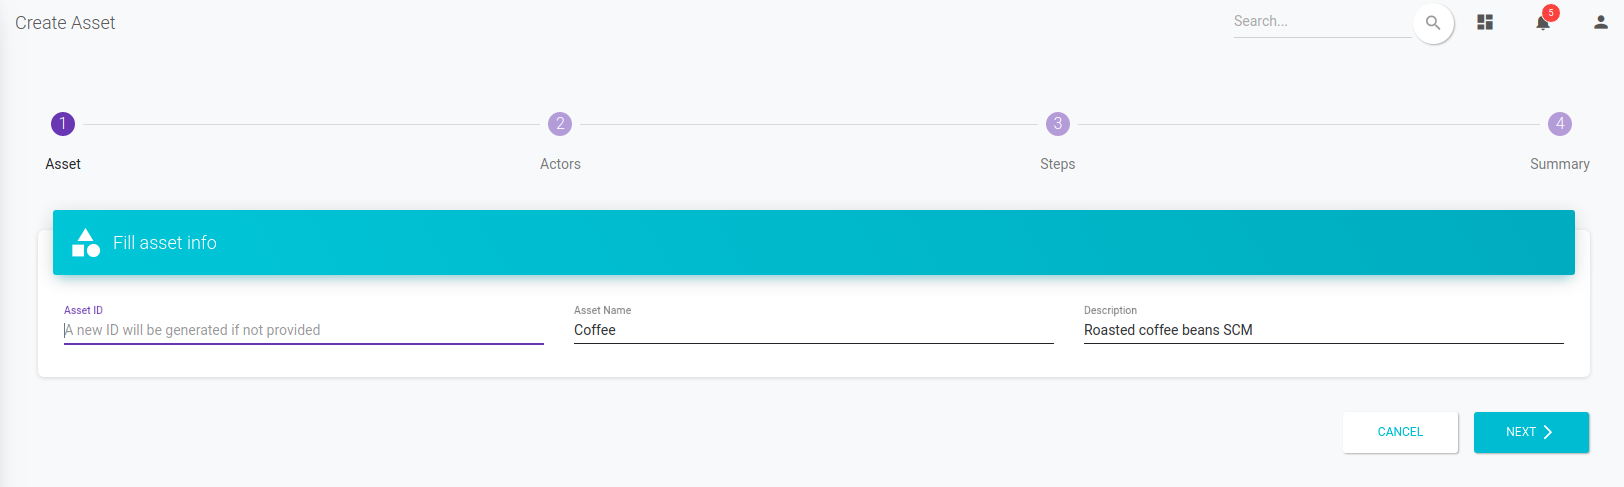
\includegraphics[scale=0.27]{images/use_example/01_create_asset_1.png}
\caption{Fill asset info.}
\label{fig:create_asset_1}
\end{center}
\end{figure}

Then the admin will add actors to the SCM informing its types. Actors can be added, updated or deleted later on, in the actors' list page.

\begin{figure}[H]
\begin{center}
  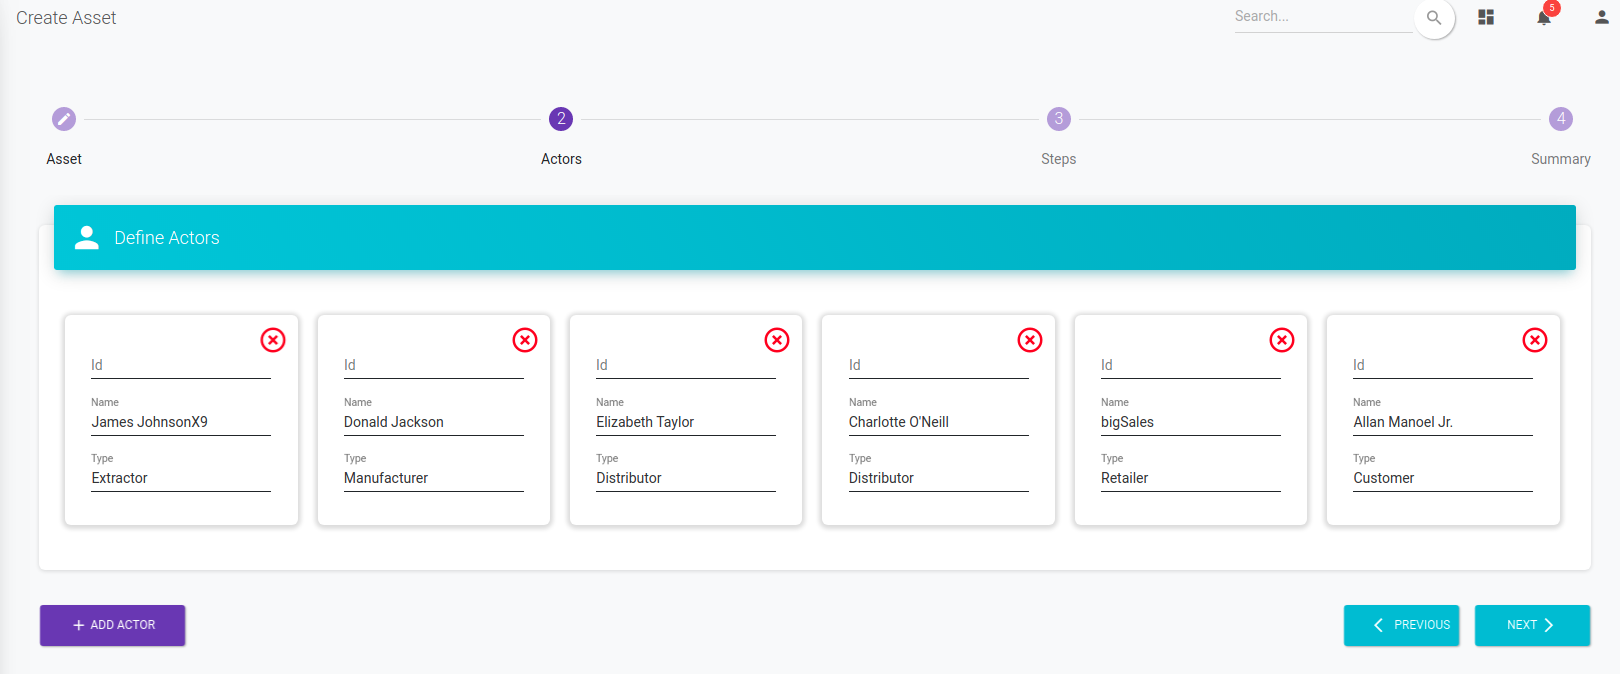
\includegraphics[scale=0.27]{images/use_example/02_create_asset_2.png}
\caption{Adding actors.}
\label{fig:create_asset_2}
\end{center}
\end{figure}


The next phase in the wizard is to define the Supply chain steps, specifying the order and binding it to the previous created actors' types:

\begin{figure}[H]
\begin{center}
  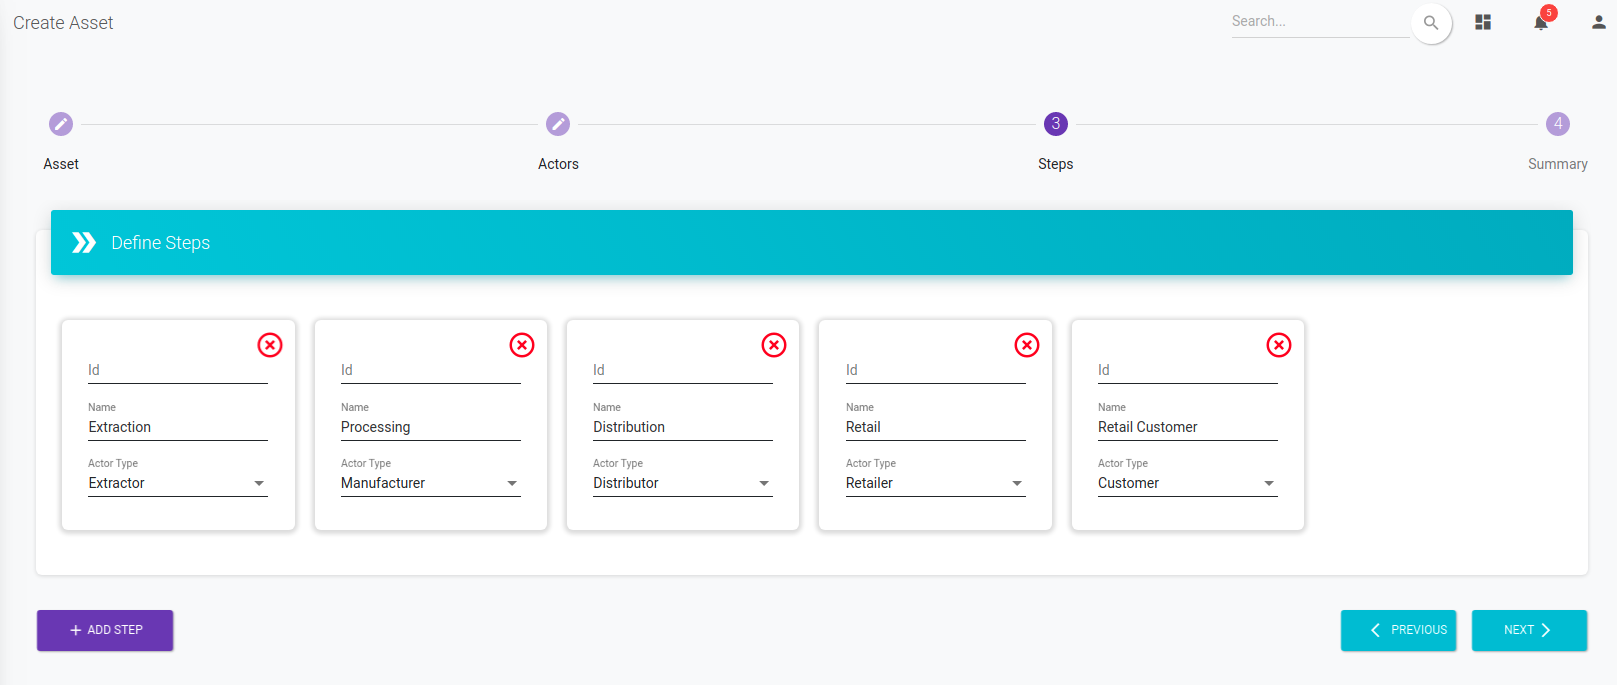
\includegraphics[scale=0.27]{images/use_example/03_create_asset_3.png}
\caption{Defining steps.}
\label{fig:create_asset_3}
\end{center}
\end{figure}

The final step, before submitting it, is to review all the information previously added in the review asset details page, under the wizard:
\begin{figure}[H]
\begin{center}
  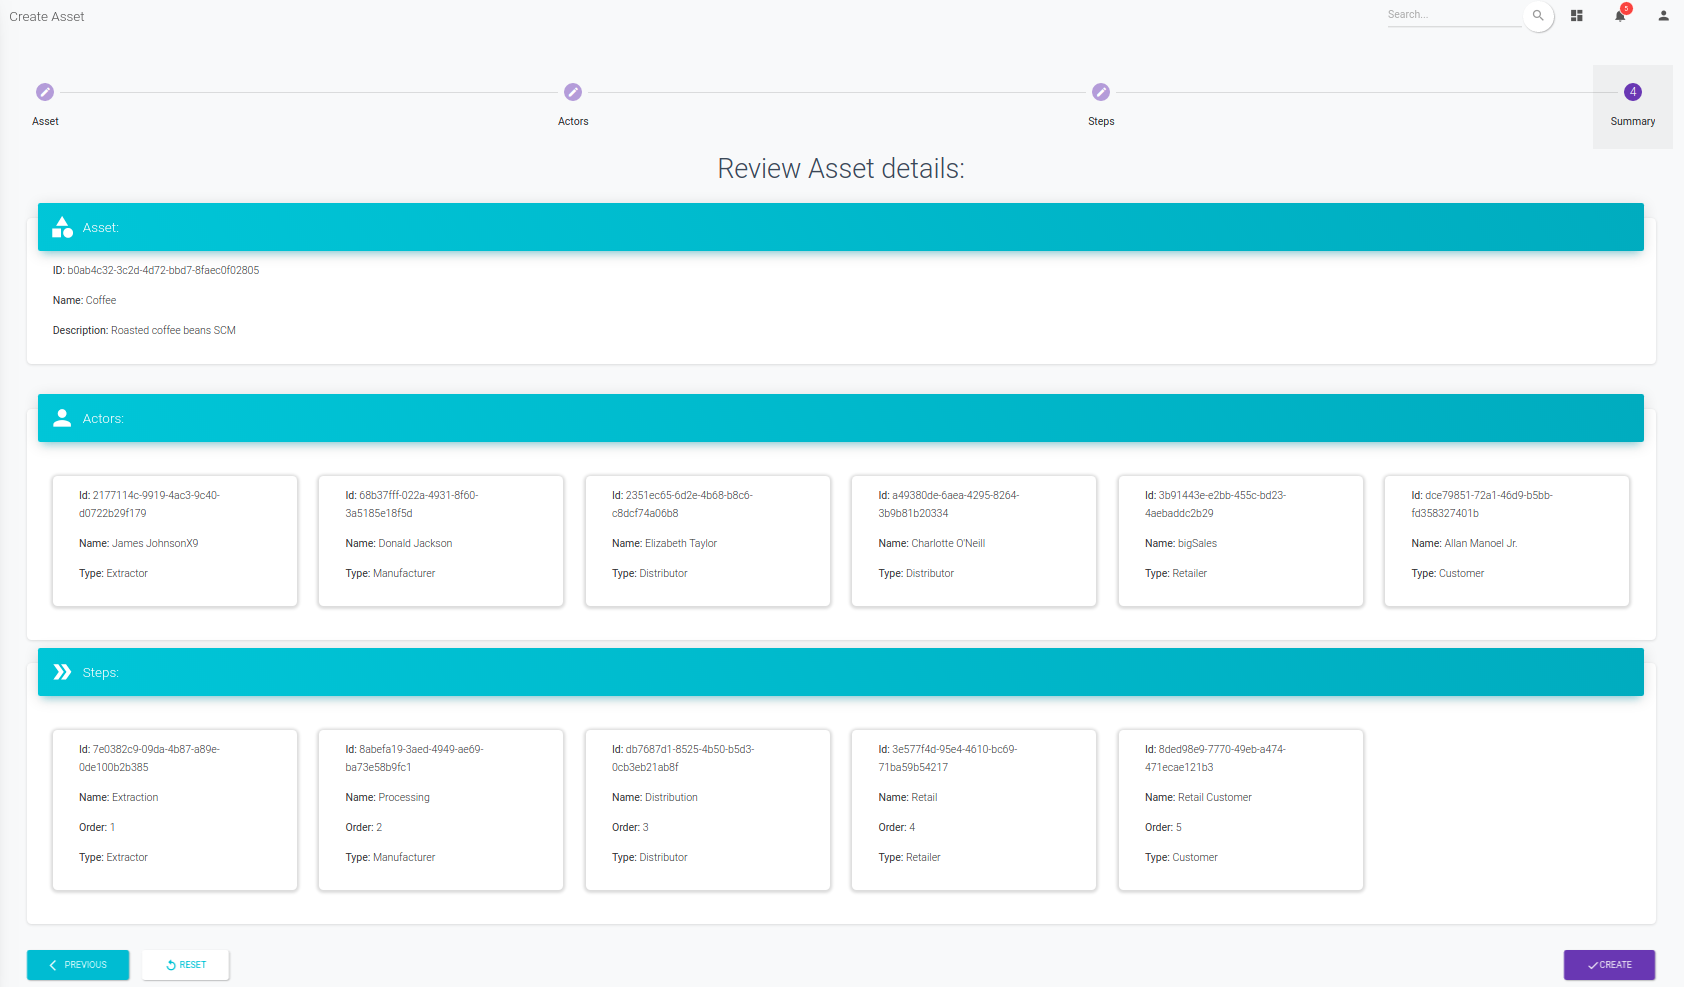
\includegraphics[scale=0.265]{images/use_example/04_create_asset_4.png}
\caption{Review asset details before submit.}
\label{fig:create_asset_4}
\end{center}
\end{figure}


Once created, the asset can be seen in the assets list, where the admin can perform crud operations by the actions items. When clicking in the asset details the current user is redirected to the asset details page where the main information about asset items, actors and steps can be seen. The card header contains a tab menu to provide navigation through these entities. 
% \begin{figure}[H]
% \begin{center}
%   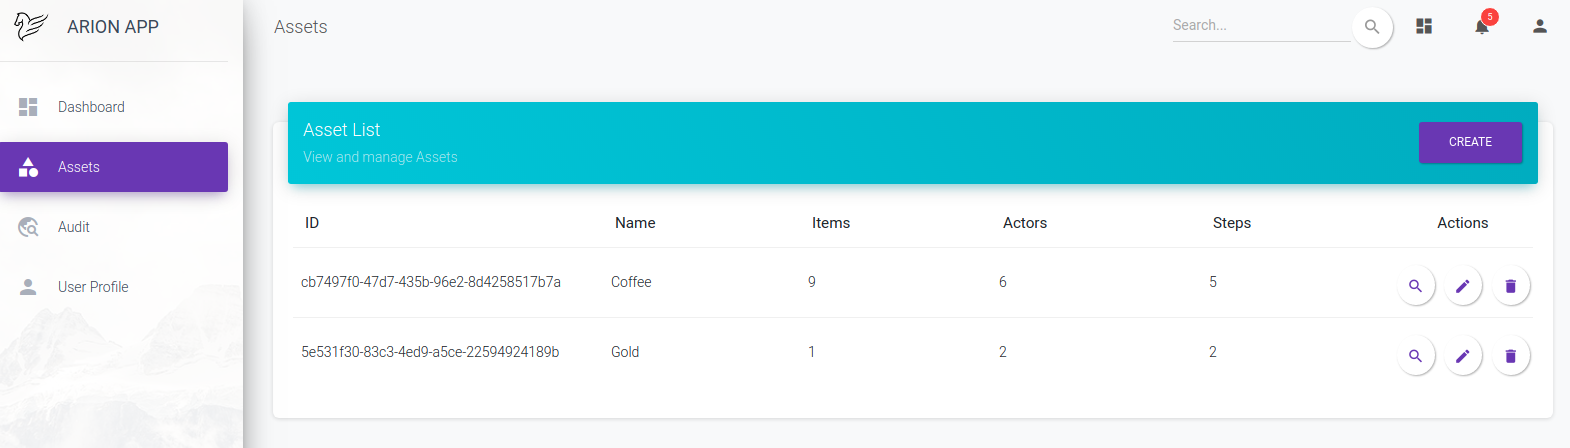
\includegraphics[scale=0.28]{images/use_example/05_asset_list.png}
% \caption{Asset list and action buttons.}
% \label{fig:asset_list}
% \end{center}
% \end{figure}



\begin{figure}[H]
\begin{center}
  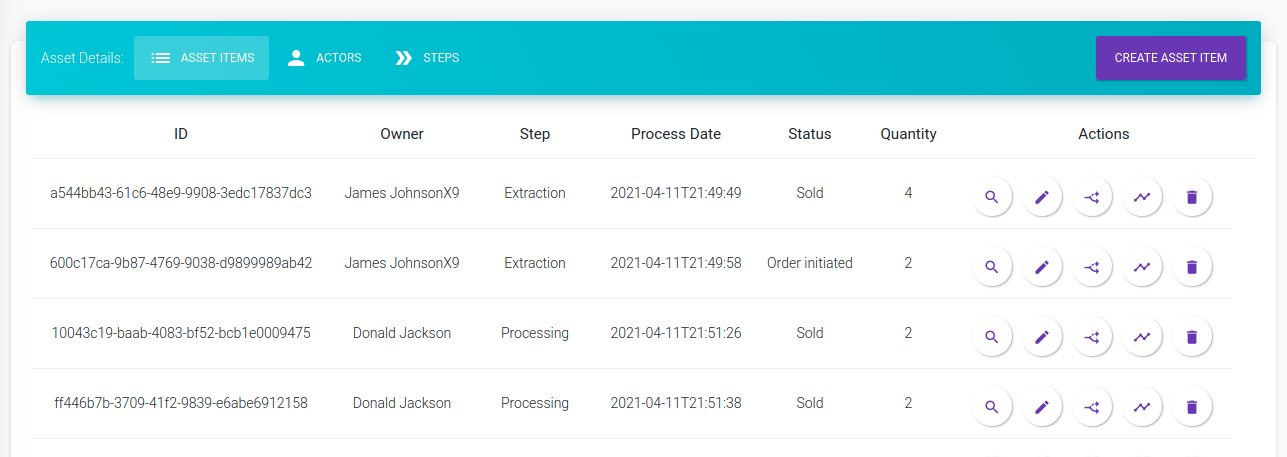
\includegraphics[scale=0.35]{images/use_example/06_asset_Item_list.png}
\caption{Asset Items list.}
\label{fig:asset_item_list}
\end{center}
\end{figure}

\begin{figure}[H]
\begin{center}
  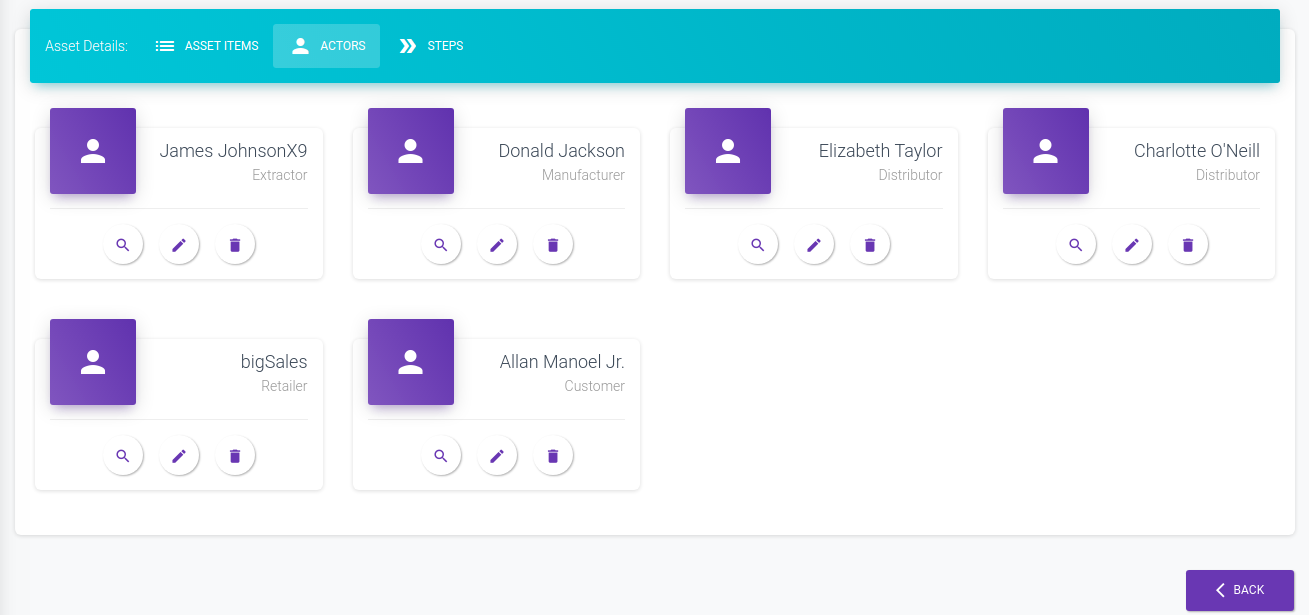
\includegraphics[scale=0.34]{images/use_example/07_actor_list.png}
\caption{Actors list.}
\label{fig:actor_list}
\end{center}
\end{figure}

\begin{figure}[H]
\begin{center}
  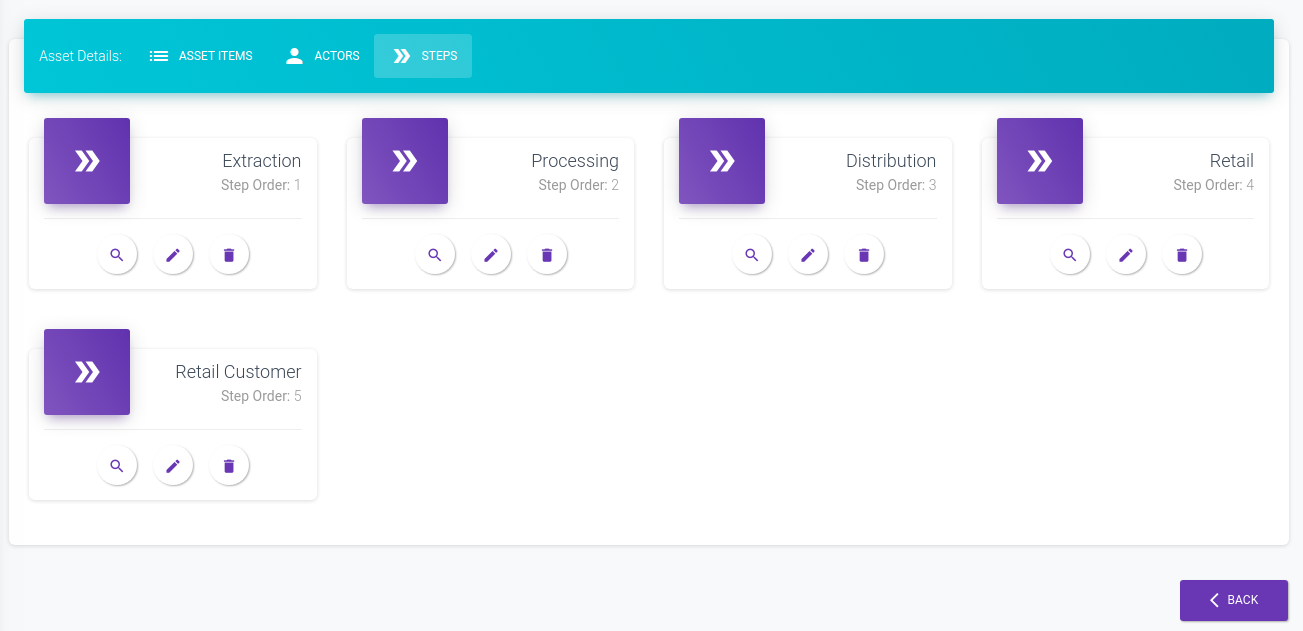
\includegraphics[scale=0.34]{images/use_example/08_steps_list.png}
\caption{Steps list.}
\label{fig:step_list}
\end{center}
\end{figure}

As an admin, there are also button actions to perform crud operations. Beyond Admins, actors responsible for the first step are allowed to create an asset item. This action will redirect the user to the create asset item form shown below. In the use case a coffee crop was harvested by the extraction company. Information about this step is added at this point. 

\begin{figure}[H]
\begin{center}
  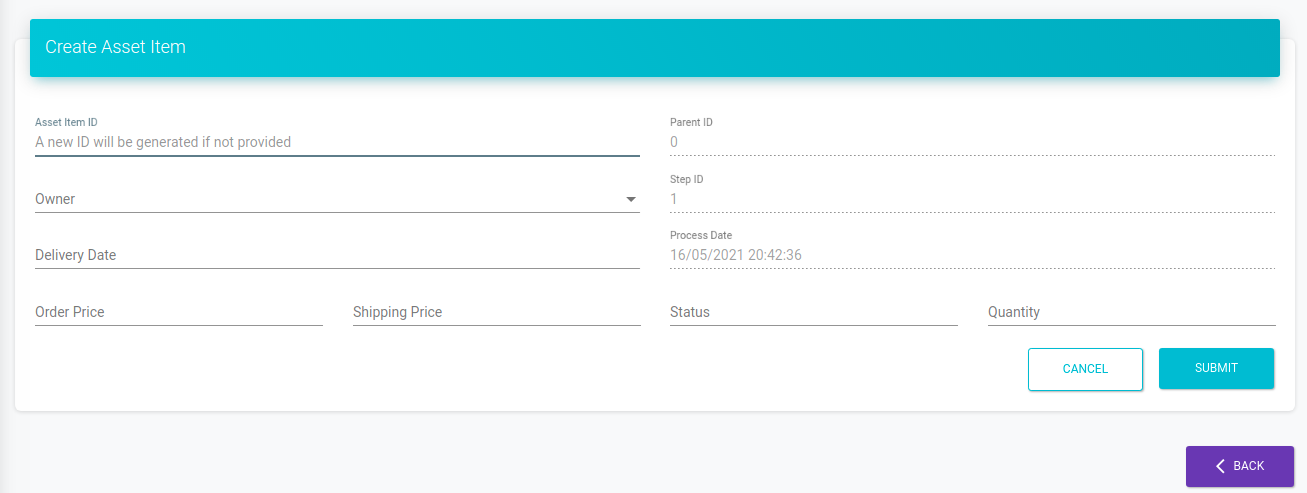
\includegraphics[scale=0.34]{images/use_example/09_create_asset_Item.png}
\caption{Create asset item form.}
\label{fig:create_asset_item}
\end{center}
\end{figure}


In the asset items list, beyond the crud actions there are also two new actions: move asset item and track asset item. The first one shows a form where the user can move an asset through the SCM steps. The user can only move this asset item to the next or the previous step in the supply chain. Move an item back to the previous step is a feature that can be used when a customer needs to return the product to whoever sold it, for example, when a product comes defective or the customer wants to exchange it. 

To the use case, the companies are using this feature to move the products towards. First, the Manufacturer company bought two lots from the same coffee crop of the extraction company. The manufacturer, after processing the products sold them into three lots. The first and the second one were sent to the first distributor company and the third to the second distributor. The first distributor delivered the first lot to the retail company and from this lot, a cup of coffee was sold to the final customer. All these actions were made from the moving asset item form below:

\begin{figure}[H]
\begin{center}
  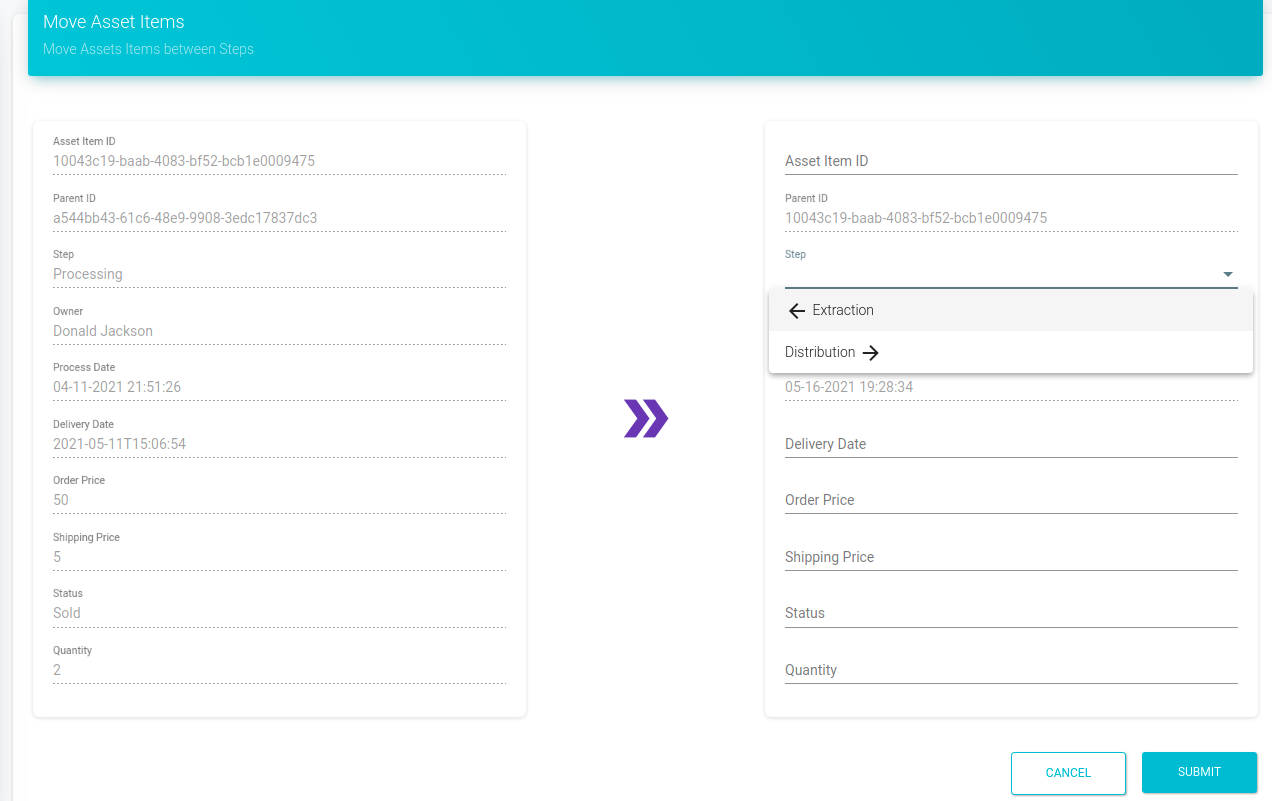
\includegraphics[scale=0.32]{images/use_example/091_move_asset_Item.png}
\caption{Move asset item form.}
\label{fig:move_asset_item}
\end{center}
\end{figure}

Track asset item displays the tracked info about the chosen asset item. It shows the children's tree of the selected element and its ancestors. The image below shows the current status of the scenario described above, by the view of the first asset item which was selected (the extracted coffee crop).

\begin{figure}[H]
\begin{center}
  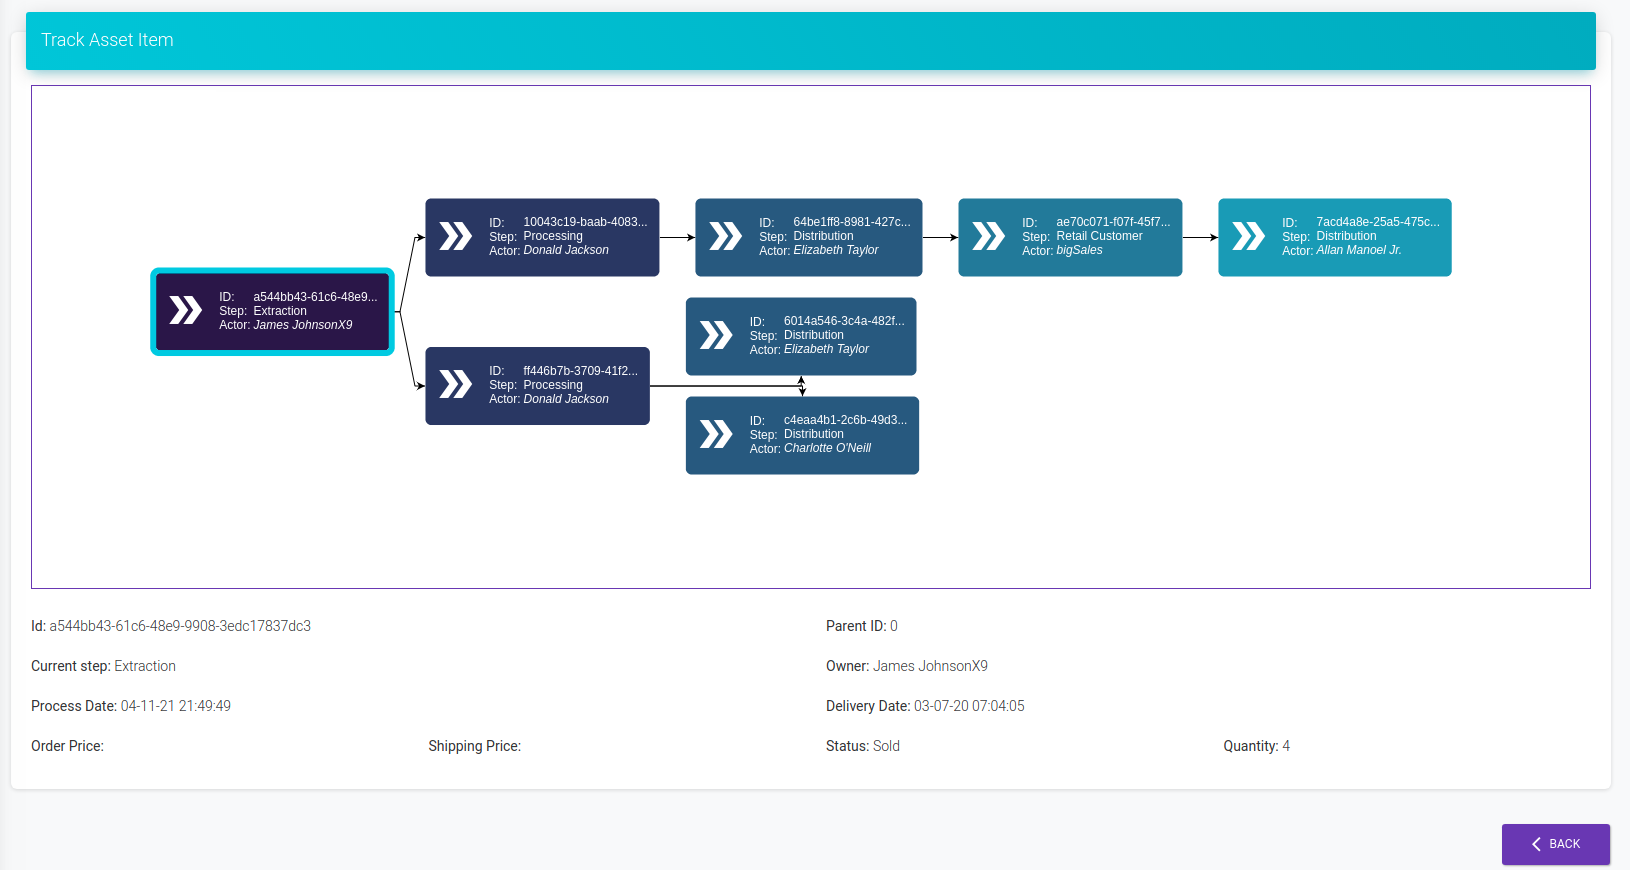
\includegraphics[scale=0.275]{images/use_example/092_track_asset_Item.png}
\caption{Track an asset item forward.}
\label{fig:track_asset_item}
\end{center}
\end{figure}

When clicking on a node in the chart, the information about the selected node is displayed under the diagram. Using this feature, the final user can track and see all the way backwards its cup of coffee has been passed. This information would be important if a problem occurred and also all the companies involved in this process could also track this information to better understand what happened, identify the possible step where a problem arose and provide input for decision making.


\begin{figure}[H]
\begin{center}
  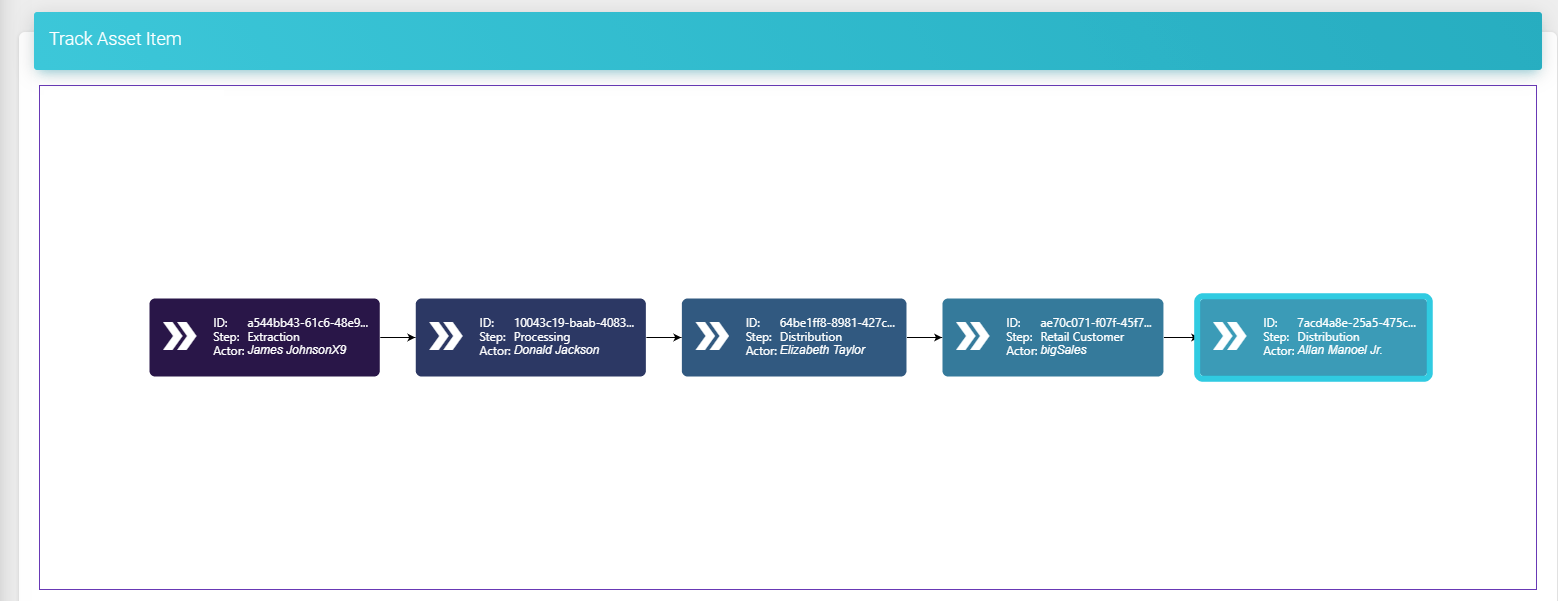
\includegraphics[scale=0.375]{images/use_example/trackbackwards.png}
\caption{Track an asset item backward.}
\label{fig:track_asset_item}
\end{center}
\end{figure}

Usage of blockchain helped to solve the problem since all the information under the blockchain is immutable, it can be audited since the information is stored and cannot be modified or deleted, the system allows anyone to check the traceability of previous records which can be achieved by arriving to the beginning of the chain. A blockchain does play a key role in traceability, as it ensures the data logged is not tampered with once it has been saved to the blockchain. 
 
 
 
 
 
\xchapter{Conclusion and Future work}{} %sem preambulo
\acresetall 
\label{chap:conclusion}

Lately, Blockchain technology has been the subject of extensive research but rarely related to supply chain traceability. Although some companies have launched pilot projects using blockchain technology to manage their supply chains, no detailed information on the technical implementation of such projects has been reported. Either way, the retail industry has the potential to use this technology to improve traceability.

Even if some properties of blockchain implementation may be beneficial for supply chain management, there are still few uses to support this claim. With so little research on this subject, it is difficult for industry stakeholders to understand exactly how blockchain technology can be used in their specific business.

This paper has presented a framework for new decentralized traceability systems based on blockchain technology. Moreover, an example scenario was given to demonstrate how it works in an enterprise supply chain. This system delivers real-time information to all supply chain members on the safety status of goods, significantly reduces the risk of centralized information systems, and brings more secure, distributed, transparent, and collaborative to the supply chain management. The Framework can significantly improve the development time of Supply Chain Management applications and provide efficiency and transparency of products in a supply chain.

While joining a blockchain consortium benefits, all stakeholders, adopting new technology such as blockchain is challenging for traditional industries due to the learning curve and cost of integrating blockchain into existing systems. Negotiating business details also takes time. In addition, the development of smart contracts must take into account quality and adaptability. Transparency and data sharing are most important in this regard. Overall, blockchain is a good option for providing traceability in supply chain management. However, the industry needs to look more closely at its risks and opportunities.

Blockchain enables end-to-end traceability by bringing a common technological language to the supply chain while allowing consumers to access the story of goods on their labels through any connected device. This characteristic has raised the need to trace products through the complex supply chain from retail back to the farm: to trace an outbreak; to verify that a product is kosher, organic, or allergen-free; or to assure transparency to consumers. Digital product information such as farm origination details, batch numbers, factory and processing data, expiry dates, storage temperatures, and shipping details are digitally connected to items. Their information is entered into the blockchain at each step of the process. All members of the business network agree upon the information acquired in each transaction. Once consensus is reached, no permanent record can be altered. Each piece of information provides critical data that may potentially reveal safety issues with the product concerned. The record created by the blockchain can also help retailers to manage the shelf life of products in individual stores and further strengthen safeguards relating to food authenticity. Across ecosystems, business model changes enabled by blockchain technology can bring strengthened trust and transparency and a new link to value exchange. Whether it is individuals seeking to complete transactions involving many parties, or enterprises collaborating across multiple organizational silos, wherever any documents or transactions must be confirmed, settled, exchanged, signed, or validated, there are usually frictions that can be avoided by using blockchain technology to unlock greater economic value.

We propose a deeper evaluation that may analyze different product types and accomplish performance tests as future work. Besides, the role permission could be applied to guarantee that only allowed users could read/write sensitive information in the blockchain. This could be made by using a flag in the additional info to show the field as public/private information or, better, use the private data collection feature provided by Hyperledger. Also, the asset item's data structure could be changed to a tree data structure for better performance results. 
%% Parte pos-textual
\backmatter

% Bibliografia
\bibliographystyle{abntex2-alf}
\bibliography{biblio}

% Apendices
\appendix

%\lipsum
% Eh aconselhavel criar cada apendice em um arquivo separado, digamos
% "apendice1.tex", "apendice.tex", ... "apendiceM.tex" e depois
% inclui--los com:
% \include{apendice1}
% \include{apendice2}
% ...
% \include{apendiceM}

\xchapter{Project Management}{}\label{app:projectManagement}

\section{Activities}{} %sem preambulo

Once determined the software architecture and its main modules, these components were divided into activities for better project management. These activities are listed below, segregated by the main modules.

\subsection{Front end}\label{sec:FrontendActivities}
\begin{itemize}
\item Create login page
\item Create application configuration module
\item Create user creation module (actors)
\item Create data entry module (forms)
\item Create data visualization module
\item Create report module
\item Create authentication service
\item Create application setup service
\item Create user creation service (actors)
\item Create data entry service (forms)
\item Create data visualization service
\item Create reporting service
\end{itemize}

\subsection{Back end}\label{sec:BackendActivities}
\begin{itemize}
\item Gateway Creation
    \begin{itemize}
    \item Create authentication endpoint
    \item Create application configuration endpoint
    \item Create user creation endpoint (actors)
    \item Create data entry endpoint (forms)
    \item Create data visualization endpoint
    \item Create report endpoint
    \end{itemize}
\item Service Creation
    \begin{itemize}
    \item Create authentication service
    \item Create application setup service
    \item Create user creation service (actors)
    \item Create data entry service (forms)
    \item Create data visualization service
    \item Create reporting service
    \end{itemize}
\item Resource Locator Creation
    \begin{itemize}
    \item Create Connector with Filesystem
    \item Create Connector with Hyperledger Blockchain
    \item Create Connector with Oracle Database
    \end{itemize}
\end{itemize}

\subsection{Hyperledger Blockchain}\label{sec:HyperledgerBlockchain}
\begin{itemize}
\item Configure the blockchain network
\item Create chaincode (Smart contract)
\item Package and install the chaincode in the network
\end{itemize}

\section{User stories}{} %sem preambulo

Table \ref{table:userStories} presents all the user stories for artifacts development, used in the system and managed according to agile methodologies.

\begin{table}[H]
\caption{\ac{SCM-BP} User Stories}
\label{table:userStories}
    \begin{tabular}{|l|p{13.5cm}|}
    \hline 
    US-1  & As an administrator, clicking “new” on the supply chain list page takes you to the chain configuration page, with empty settings (no phases, sub-phases, and fields).\\
    \hline 
    US-2  & As an administrator, clicking “edit” on the supply chain list page takes you to the chain configuration page, with the settings filled in (with phases, sub-phases, and fields already registered). \\
    \hline
    US-3  & As an administrator, when clicking delete on the supply chain list page, a modal should appear requesting deletion confirmation.\\
    \hline
    US-4  & As an administrator, when clicking  confirm deletion on the supply chain list page, an alert should appear stating the deletion result: alert-success or alert-danger.\\
    \hline
    US-5  & As an administrator, on the creation or editing screens of a chain, the administrator must tell from each section which user types can enter information in that section.\\
    \hline
    US-6  & As an administrator, when clicking on the User List page redirects to the user creation page with its empty settings.\\
    \hline
    US-7  & As an administrator, on the user creation page, the admin have to enter the type of user (Admin, Producer, Manufacturer, Distributor, Wholesaler, Retailer, End User).\\
    \hline
    US-8  & As an administrator, clicking “edit” on the User List page takes you to the user creation page, with the settings filled in (with the previously entered data).\\
    \hline
    US-9  & As an administrator, when clicking delete on the User List page, a modal should appear asking for deletion confirmation.\\
    \hline
    US-10 & As an administrator, when clicking confirm deletion on the User List page, an alert should appear stating the deletion result: alert-success or alert-danger.\\
    \hline
    US-11 & As a "Member" User (Admin, Producer, Manufacturer, Distributor, Wholesaler, Retailer), clicking Move Asset redirects to the information entry page in the chain.\\
    \hline
    US-12 & As a "Member", each user can only enter information regarding the allowed phase in the access rules (e.g., a distributor cannot enter exploration information) as defined in use case 5.\\
    \hline
    US-13 & As any user (Admin, Member, or End User), clicking Track Asset will take you to a page with a list of all assets paged and filtered by date in descending order (most current to oldest).\\
    \hline
    US-14 & As any user (Admin, Member, or End User), by clicking on “Track Asset”, the user can enter an Id in the input search to search.\\
    \hline
    US-15 & As any user (Admin, Member, or End User), by clicking on “Track”, the user will go to a page with all information of the respective asset, from its conception to the current state.\\
    \hline
    \end{tabular}
\end{table}
\section{Non-functional requirements}{} %sem preambulo

\begin{table}[H]
\caption{Non-functional requirements of \ac{SCM-BP}}
\label{table:rnf}
\begin{tabular}{|p{3cm}|p{12cm}|}
\hline
NF-1: Usability & The available product, corresponding APIs and documentation should be clear enough to allow for the developers to perform the implementation.\\
\hline
NF-2:  \newline Performance &  \textbf{Speed and latency}:  The throughput and latency on Hyperledger have already been tested, and the throughput is not expected to be as high as in a centralized data system. But, overall, the time to synchronize the information from one company to another might increase; The goal is to make the product be as fast as needed to support the businesses, even if it does not have better performance than other alternatives, since what the target here is the addition of new functionalities (shared ledger); \newline
\textbf{Precision and accuracy}: The product shall record the data just as it was entered, and predictions as to whether a product has any mismatching entries shall always be justifiable; \newline
\textbf{Reliability and availability}: The product shall not always be available unless all of the nodes fail at once, which is almost impossible, unless a coordinated attack were to happen; If some of the nodes happen to fail, the response time of the system might be lower than expected; \newline
\textbf{Scalability}: The product should scale to hundreds of companies, which would require a similar number of nodes;
\\
\hline
NF-3:  \newline Maintainability and portability & The product is expected to run on Linux based systems, compatible with the Docker, nodejs and golang versions that Hyperledger Fabric uses. More specifically, Oracle Cloud services have servers with the required setup for this. Creating new nodes or moving an existing one should be an easy process, without much complication, other than starting the node software on the environment, and closing an existing one, if needed. \\
\hline
NF-4: Security & 
\textbf{Privacy}: The system must ensure appropriate visibility of transactions and products, which might be privacy sensitive; sharing some data would pose a threat or could possibly have negative effects for some of the companies; otherwise, transactions should also be secure, authenticated and verifiable; \newline
\textbf{Immutability}: No one can make changes to the contents of the ledger;\newline
\textbf{Authorization}: All changes to any data should be approved by the people that possess the data or will be affected by these changes directly. A shipment delivery transaction should, for instance, be approved by both the person delivering and the person receiving the shipment. \\
\hline
\end{tabular}
\end{table}
\section{User creation fields}{} \label{app:userCreationFields}

\begin{table}[H]
\centering
\caption{User creation service fields}
\begin{tabular}{|p{3cm}|p{12cm}|}
\hline
Field & Input Value \\ 
\hline
User ID & Create a unique identifier for this user's login user name. Duplicated Id is not allowed. \\ 
\hline
First name & Enter the user's full first name. \\ 
\hline
Last name & Enter the user's last name. \\ 
\hline
Title & Enter a title or job description, or select one from the list. \\ 
\hline
Department & Select the user's department from the list. \\ 
\hline
Password & Assign a password to the user. This password can be permanent or temporary. \\ 
\hline
Password needs reset & Select this check box to require the user to change the password during the first login. \\ 
\hline
Locked out & Select this check box to lock the user out of the instance and terminate all their active sessions. \\ 
\hline
Active & Select this check box to make this user active. Only the administrator sees inactive user in: 
\begin{itemize}
\item Lists of users 
\item The selection list on reference fields (magnifying glass icon) 
\item The auto-complete list that appears when you type into a reference field.
\end{itemize} \\ 
\hline
Web service access only & Select this check box to designate this user as a non-interactive user. This field is available with Non-Interactive Sessions. \\ \hline
Internal Integration User & Select this check box to designate this user as an internal integration user. \\ 
\hline
Date format & Select the user's preferred format for dates. \\ 
\hline
Email & Enter the user's email address. \\ 
\hline
Notification & Select the type of notification to send to this user. The default is Email. \\ 
\hline
Time zone & Select the user's time zone. \\ 
\hline
Business phone & Enter this user's business phone number. \\ 
\hline
Mobile phone & Enter this user's mobile phone number. \\ 
\hline
Photo & Attach a photo of the user, if appropriate. \\ 
\hline
Geolocation tracked & Select the check box to enable location tracking. \\ 
\hline
Location & Select the user's usual location. This field is visible when geolocation is active. \\ 
\hline
\end{tabular}
\end{table}

\xchapter{Data Structure}{} %sem preambulo
%\xchapter{Data Structure}{} %sem preambulo

%\section{Data Structure}{} %sem preambulo

\begin{figure}[H]
\begin{center}
  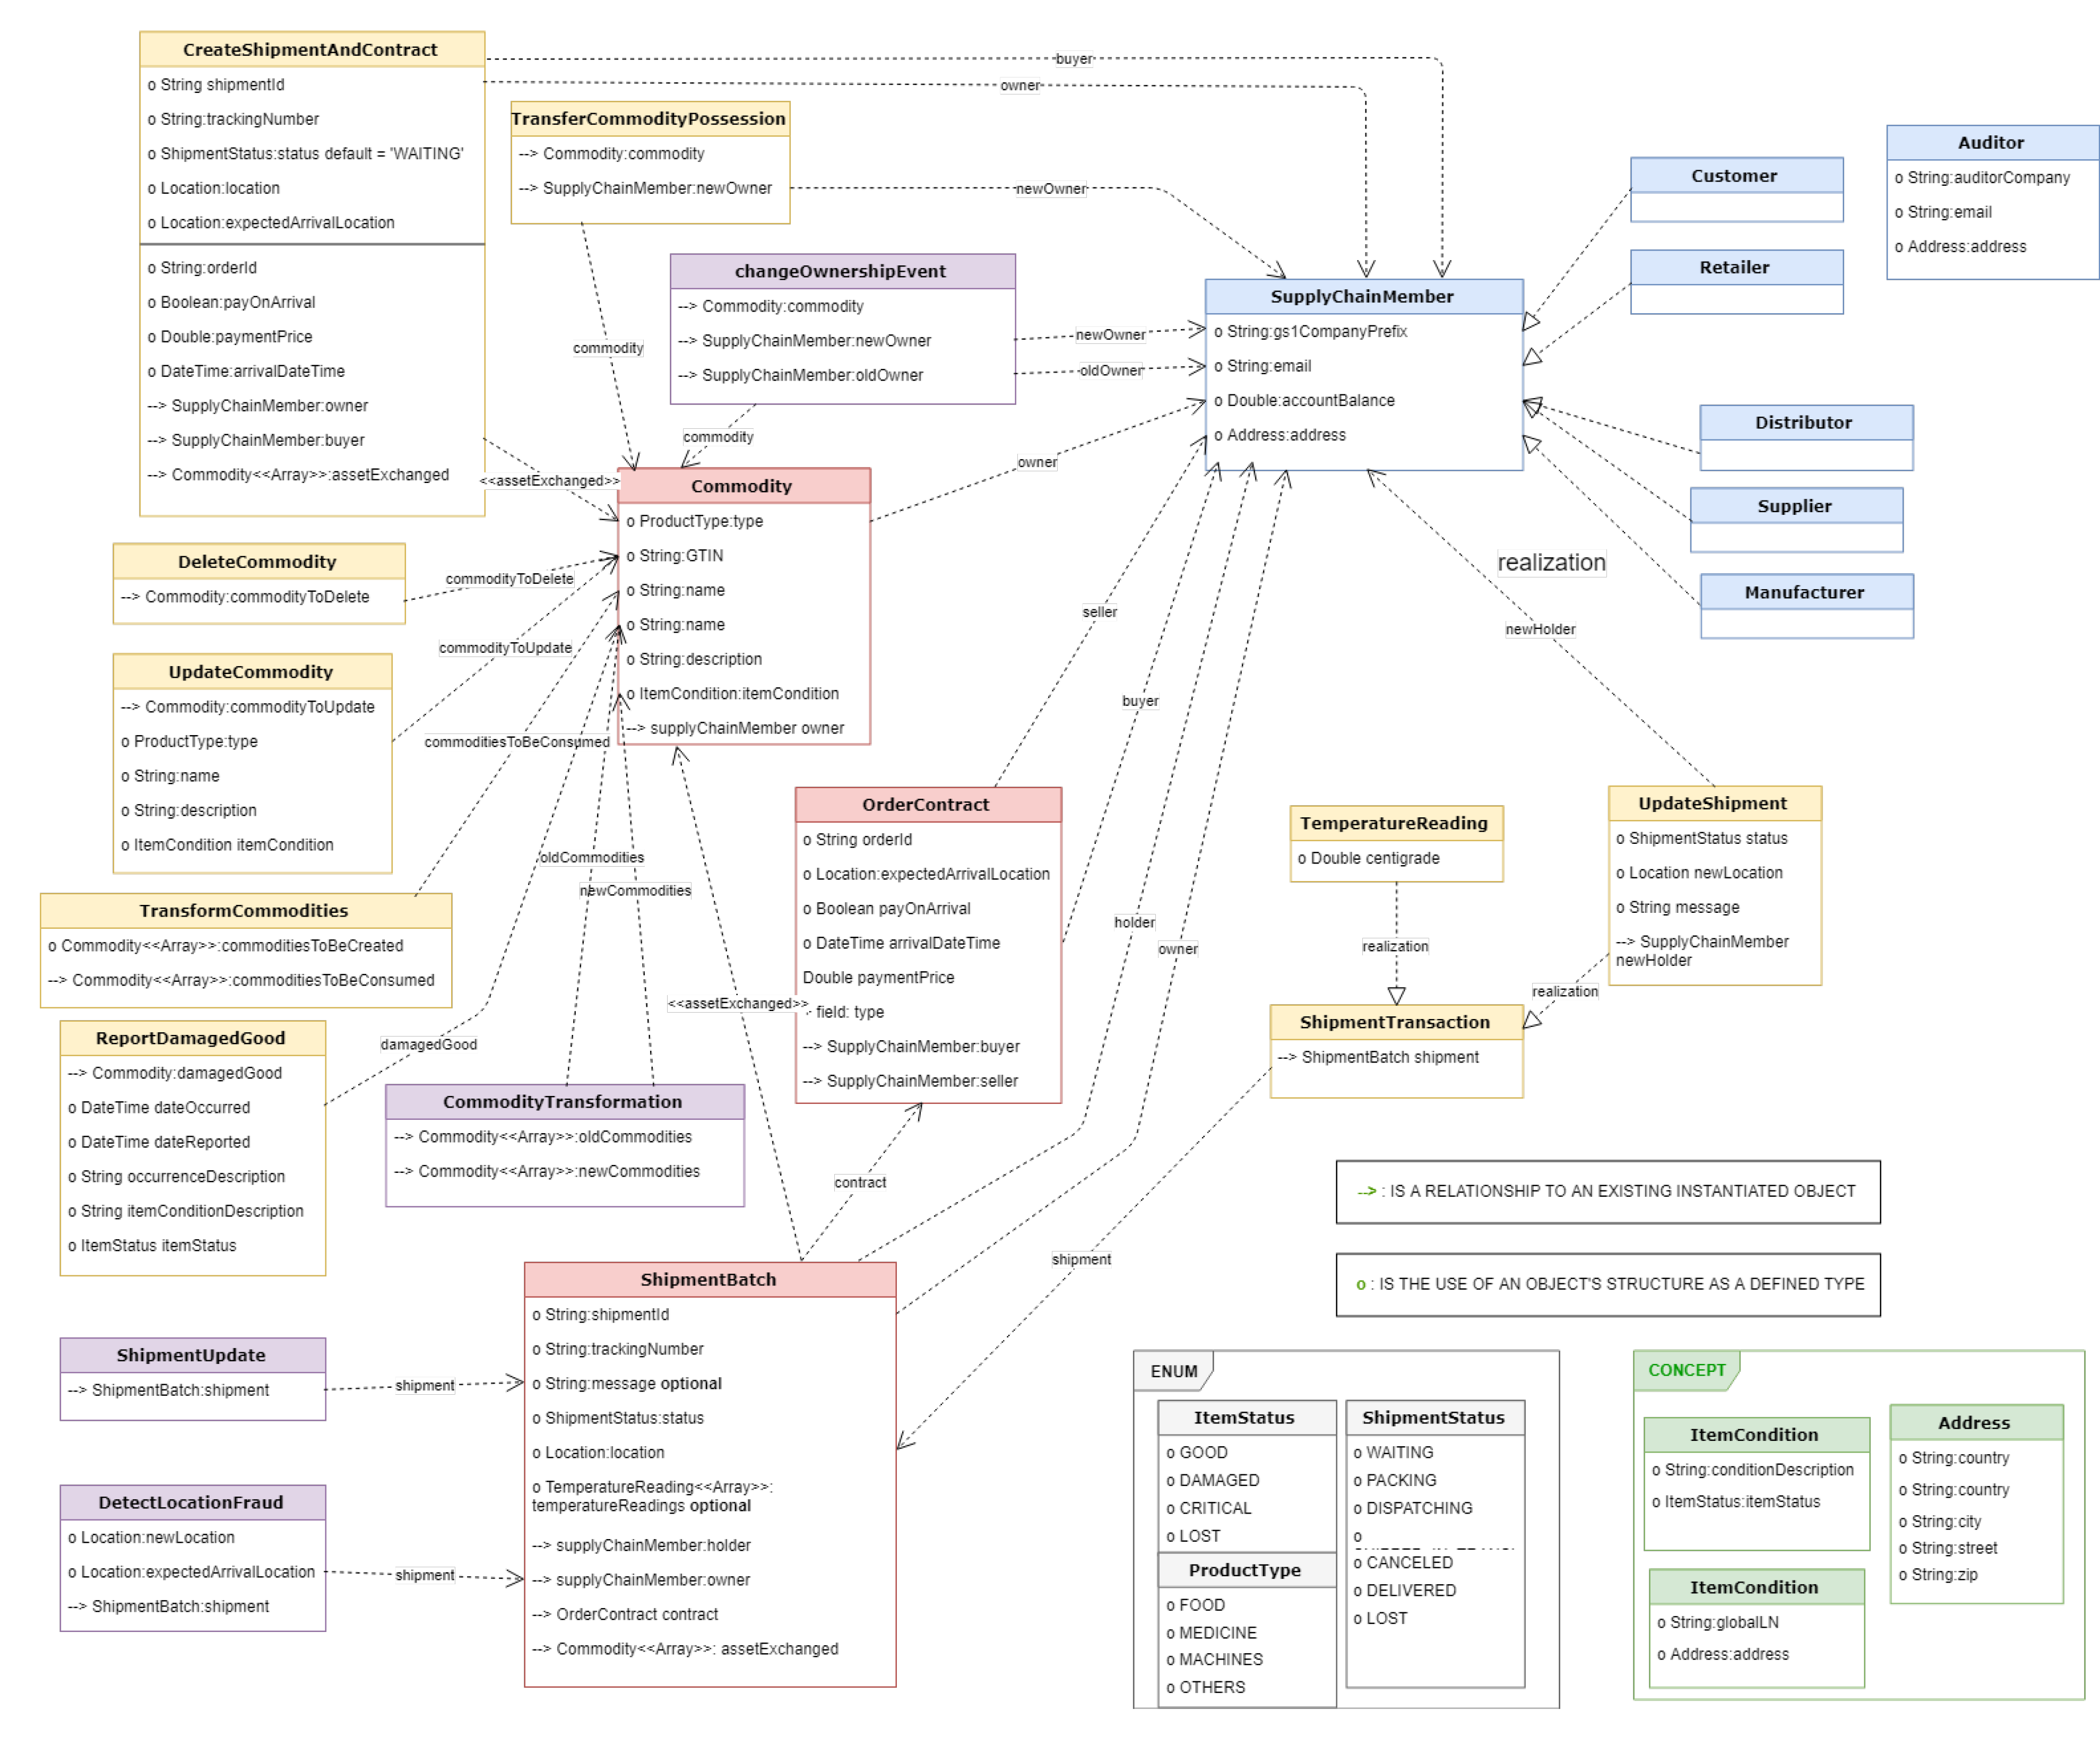
\includegraphics[scale=0.95]{images/classDiagram.png}
\caption{\ac{SCM-BP} data structure}
\label{fig:dataStructure}
\end{center}
\end{figure}

\xchapter{Frontend Screens}{}
\begin{figure}[H]
\begin{center}
  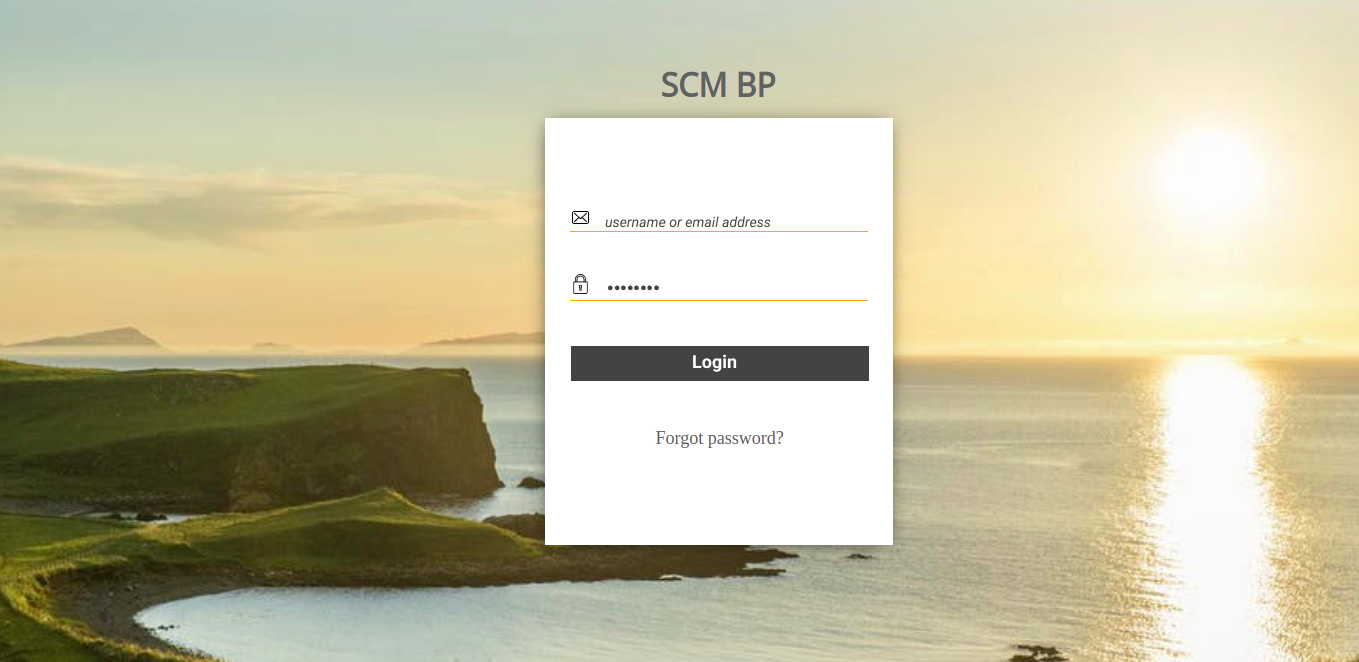
\includegraphics[scale=0.33]{images/login.png}
\caption{Login screen.}
\label{fig:login}
\end{center}
\end{figure}

\begin{figure}[H]
\begin{center}
  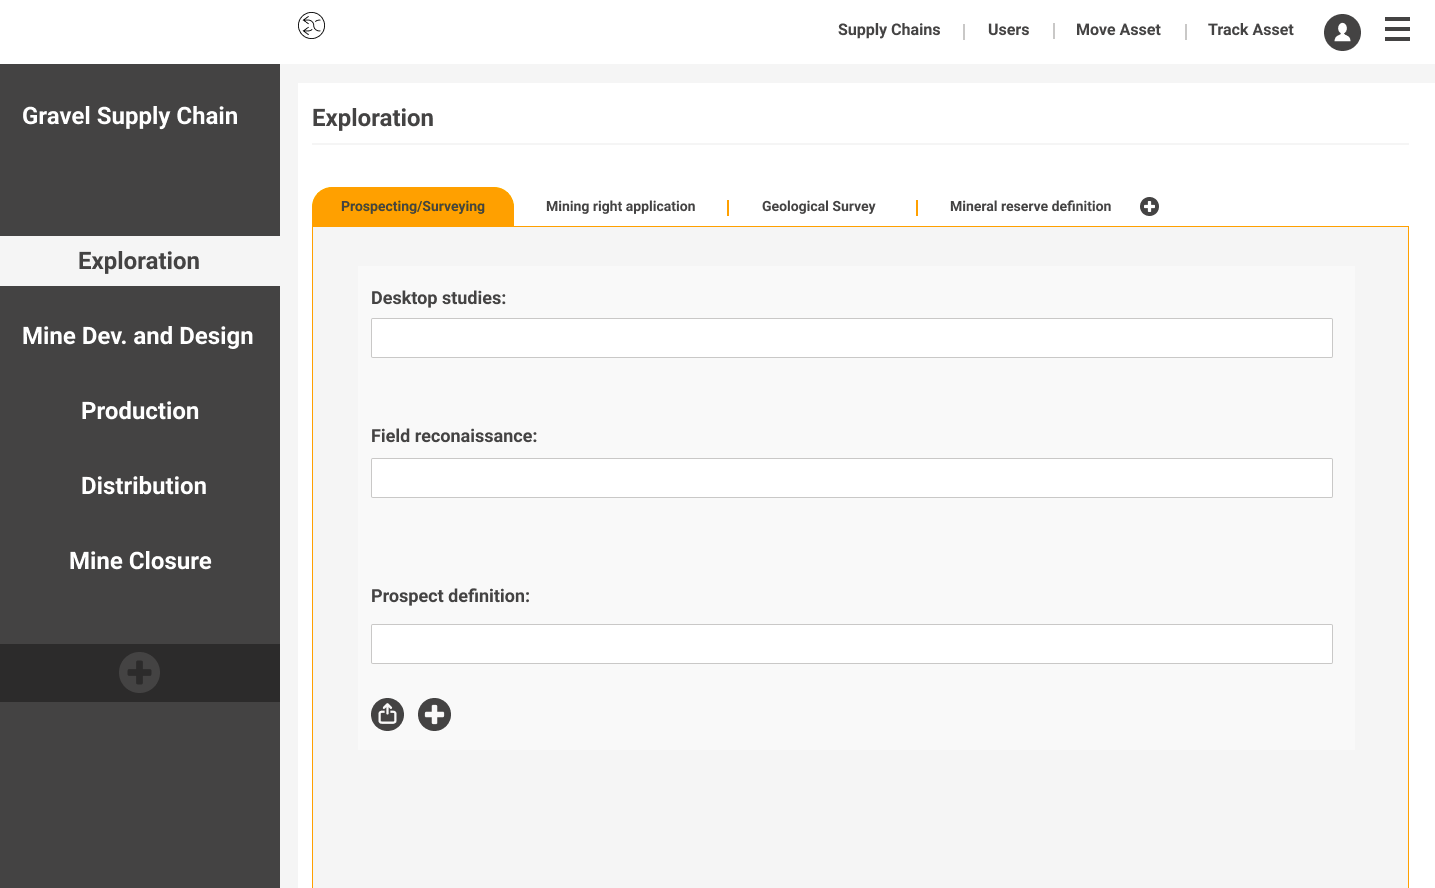
\includegraphics[scale=0.31]{images/configure_scm.png}
\caption{Setup screen.}
\label{fig:configure}
\end{center}
\end{figure}
%% Fim do documento
\end{document}
%------------------------------------------------------------------------------------------%
